\chapter{Introduction}
\thispagestyle{firstpage}
\onehalfspacing
\setcounter{page}{1}

%%% NOUVELLE SECTION
\par Si l’évolution peut avoir plusieurs définitions dans le dictionnaire, elle a une définition très spécifique dans l’univers de la biologie. En effet, l'évolution se réfère à la modification progressive du monde vivant au fil du temps. L’évolution est un mécanisme complexe et permet la diversité de la vie sur Terre. Elle peut se caractériser par plusieurs sous-notions comme la notion d’hérédité, d’adaptation, de sélection, de coévolution, de mutation ou encore de spéciation. Ces grandes notions vont être importantes pour la suite de l’introduction : la génétique, l’étude des gènes, et génomique, celle des génomes. Dans les prochains chapitres introductifs, nous détaillerons ce que sont les gènes et génomes, la diversité animale, et brièvement la communication cellulaire. 

%%% GENES ET GENOMES
\section{Gènes et génomes}\label{genes}
\par Les gènes sont des fragments d’ADN (acide désoxyribonucléique) qui comportent l’information génétique de chaque organisme vivant. L’ADN mitochondrial est stocké principalement au niveau du noyau de la cellule pour les organismes eucaryotes (à la différence des organismes procaryotes, donc sans noyau où l’ADN est retrouvé concentré en région que l’on appelle le nucléoïde). Les gènes sont transmis d’une génération à une autre, mais sont soumis à des modifications aussi appelées « mutations » de leur séquence nucléotidique (succession d’éléments : adénine (A), cytosine (C), guanine (G) et thymine (T)). Pour être traduit en protéine, la séquence nucléotidique d’un gène se lit par codon, une suite de 3 nucléotides. Chaque combinaison de codon correspond à un acide aminé. Il existe 20 acides aminés communs à l’ensemble du vivant \parencite{ambrogelly_natural_2007}. Une suite d’acides aminés commençant par un codon initiateur et se finissant par un codon terminal deviendra sera dans un premier temps transcrit en ARNm (acide ribonucléique messager) puis traduit en protéine par le biais de la traduction réalisée par un ribosome.
\par La transcription a lieu dans le noyau de la cellule, et transcrit donc la séquence nucléotidique en séquence complémentaire. Il est important de préciser qu’un même gène peut conduire à une multitude de protéines \parencite{breathnach_organization_1981}. En effet, les gènes sont constitués de sous-parties : d’un promoteur (partie initiatrice de la transcription), d’exons (parties codantes de l’ADN, elles vont aider à déterminer la structure de la protéine) et d’introns (parties non codantes de l’ADN, elles vont jouer un rôle dans la régulation de l’expression génique) \parencite{scherrer_pre-messenger_1979, keren_alternative_2010, shaul_how_2017}. Chez les eucaryotes, avant que l’ARNm ne soit traduit en protéines, il va être édité et ce phénomène s’appelle la maturation. Les introns vont être épissés, et les exons conservés. Un même gène peut avoir différentes combinaisons d’exons assemblés, ce qui peut conduire à avoir plusieurs protéines différentes (Figure \ref{fig:1_genetoprotein}).
\par Comme on a pu le voir, les gènes sont des petits éléments complexes, mais indispensables à un organisme. L’ensemble des gènes constitue le génome. 

\begin{figure}[H]
    \centering
    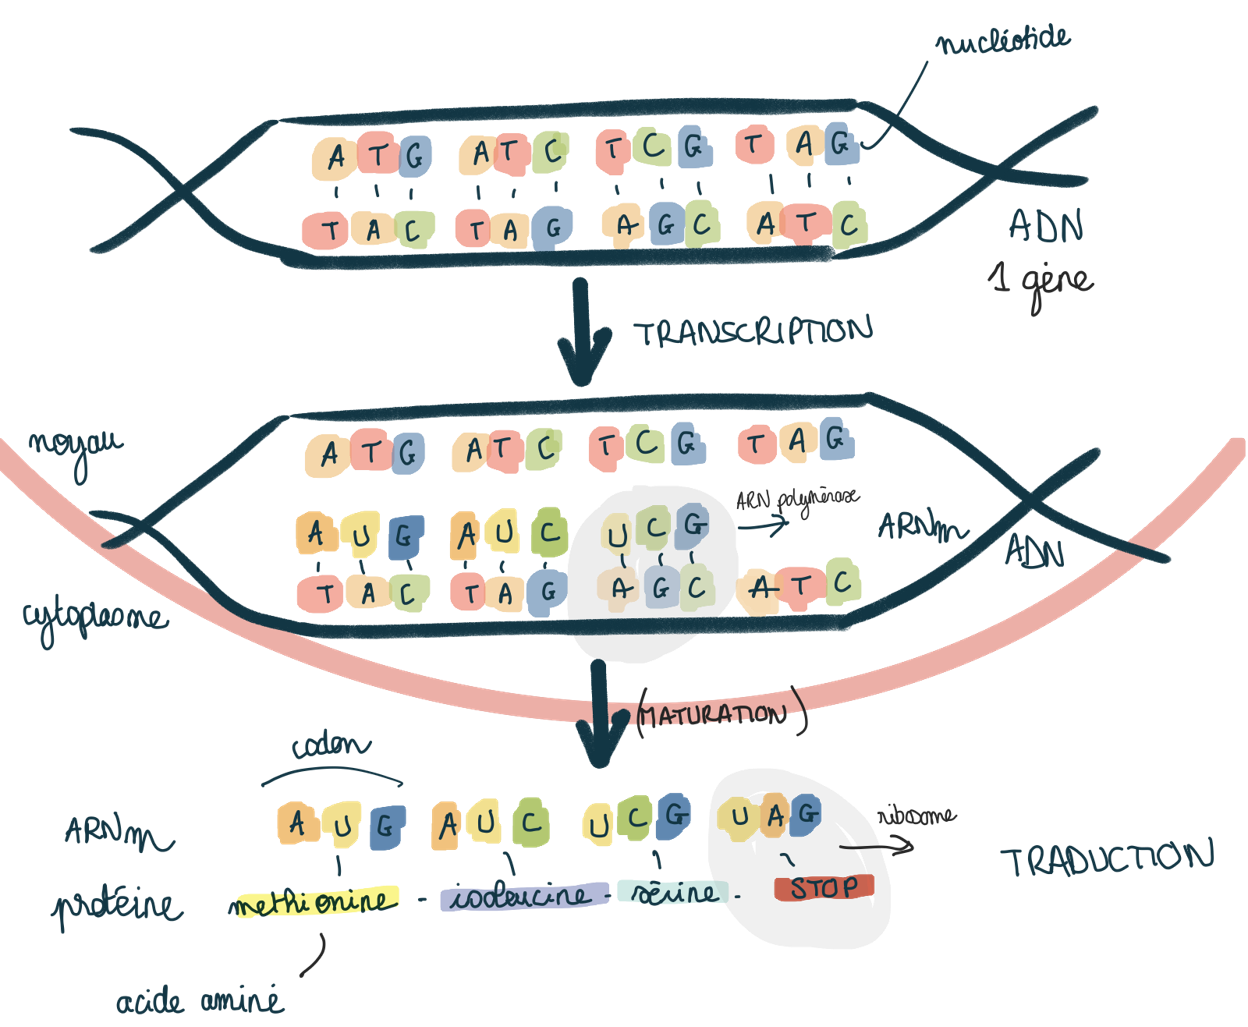
\includegraphics[width=1\textwidth]{figures/corps/figure1.png}
    \caption{Schéma d'un gène à une protéine}
    \label{fig:1_genetoprotein}
\end{figure}
Légende : Les différentes étapes d’un gène à une protéine sont représentées à l’exception de la maturation (épissage alternatif).\\

%%% EVOLUTION DES GENES, MUTATION DELETIONS INSERTIONS
\subsection{Évolution des gènes : mutations, délétions, insertions}\label{mutations}
\par L'ADN peut subir des changements de différentes manières. Tout d'abord, il y a les mutations, qui peuvent être spontanées, se produisant lors de la transmission de l'information génétique à la descendance, ou environnementales, résultant d'altérations dues à des facteurs extérieurs tels que les virus et le soleil, entre autres. Ces mutations affectent la séquence de nucléotides et peuvent entraîner des conséquences plus ou moins graves en fonction de leur nature.
\par Une mutation peut être une substitution d’un nucléotide par un autre. En fonction du nucléotide touché, elle peut avoir plus ou moins de conséquences. Le code génétique est doté de quelques redondances concernant la traduction des acides aminés. Par exemple, la sérine est un acide aminé codé par 6 codons différents (UCU, UCC, UCA, UCG, AGU et AGC). Si la séquence est initialement UCG, et que la substitution a lieu sur le 3ème nucléotide de la séquence : il n’y aura pas d’impact sur la traduction du codon, quelle que soit la substitution. Cette mutation est dite silencieuse. Si la substitution a lieu sur le 2ème nucléotide, de telle façon à former UAG, on obtient donc un codon stop, ce qui veut dire que le ribosome n'ira pas au-delà lors de la traduction. La protéine ne sera donc pas celle initialement prévue, possiblement tronquée et non fonctionnelle. Cette mutation est dite non-sens. Et enfin si la substitution a lieu sur le 1ème nucléotide, de telle façon à former GCC, on obtient un nouvel acide aminé qui est l'alanine. Cette mutation est dite faux sens car la protéine finale sera impactée par ce changement d'acide aminé (Figure \ref{fig:2_mutations}).
\par Une mutation peut aussi prendre la forme d'une insertion ou d'une délétion, c'est-à-dire l'ajout ou la suppression d'un nucléotide dans la séquence d'ADN. Étant donné que la séquence se lit en codons, cela perturbera le "cadre de lecture" si un ou plusieurs nucléotides (non multiple de 3) sont ajoutés ou supprimés. Le cadre de lecture détermine comment les codons seront lus par le ribosome lors de la traduction (Figure \ref{fig:2_mutations}). 
\par Il existe également la recombinaison génique qui est un déplacement d’une région d’ADN vers une autre. Lors de ces recombinaisons, il se peut que la séquence soit également dupliquée \parencite{sasaki_genome_2010, stewart_homologous_2022, syeda_recombination_2014}. Des copies de gènes ou des copies de séquence sont alors ajoutées dans la séquence, que l’on appelle des duplications segmentales. Lorsqu’il s’agit de gène entièrement dupliqué, différents scénarios peuvent avoir lieu. Le gène dupliqué peut garder la fonction initiale du gène original. Le gène peut acquérir une nouvelle fonction proche, voire une spécialisation (spatio-temporel) au gène original. Mais il peut également se pseudogéniser, c’est-à-dire devenir non fonctionnel par une altération de sa séquence. 
\par Les mutations ont donc un effet direct sur la séquence nucléotidique, mais également sur la protéine et la fonctionnalité de celle-ci, effet qui peut être avantageux ou désavantageux \parencite{long_origin_2003}. Les duplications sont également un moteur de l’évolution. L’exemple de la famille des globines peut en attester \parencite{weatherall_molecular_1976}. En effet, les duplications des globines ont permis aux vertébrés de s’adapter à différents environnements ou à des contraintes physiologiques. 

\begin{figure}[H]
    \centering
    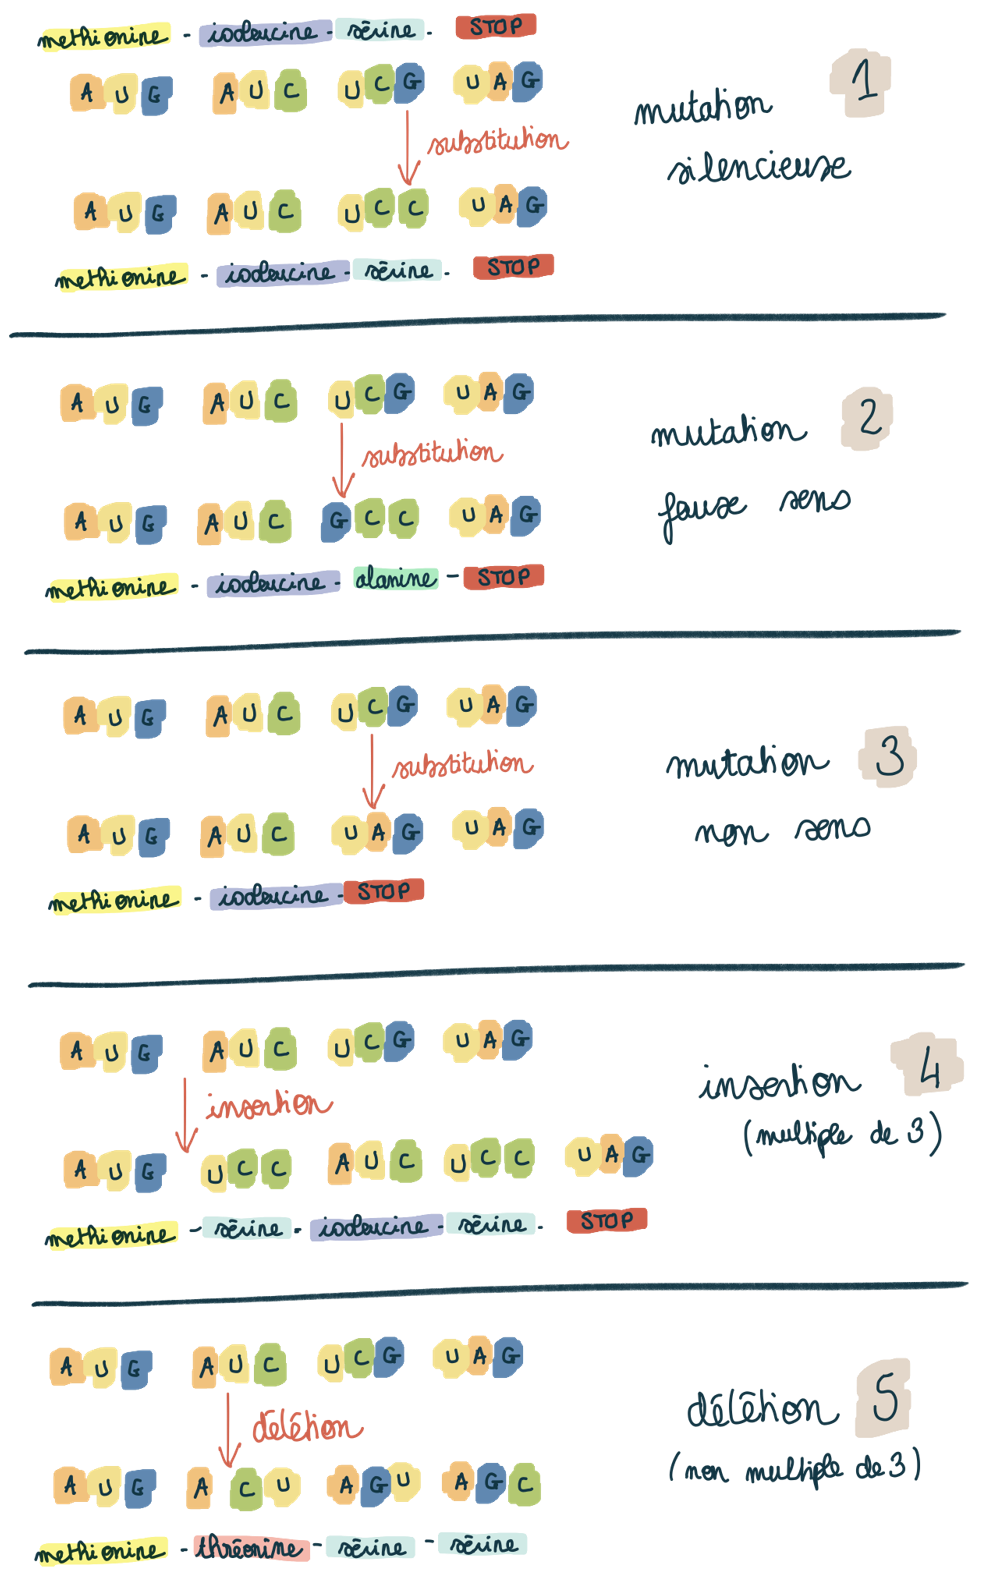
\includegraphics[width=0.85\textwidth]{figures/corps/figure2.png}
    \caption{Différents types de mutations}
    \label{fig:2_mutations}
\end{figure}
Légende : Représentation des mutations silencieuses, faux sens, non-sens, des insertions et délétion à partir d’une même séquence initiale. \\

\par Les duplications segmentales sont des événements à échelle restreinte, mais il existe également une autre forme de duplication, la duplication complète du génome.


%%% DUPLICATION COMPLETE DE GENOME
\subsection{Duplication complète de génome}\label{wgd}
\par La duplication de génome (Whole Génome Duplication en anglais, WGD) est un événement de polyploïdisation, c’est-à-dire une duplication du nombre de chromosomes. La polyploïdisation est très courante dans le règne des plantes, puisque environ 70\% des angiospermes ont eu au moins un événement de polyploïdisation \parencite{masterson_stomatal_1994, soltis_polyploidy_2009}.
\par Les premières études démontrant des phénomènes de duplication ancestrale de génome chez les plantes date des années 2000 chez \textit{Arabidopsis Thaliana} \parencite{blanc_recent_2003, bowers_unravelling_2003, the_arabidopsis_genome_initiative_analysis_2000} et concernant le règne des animaux, les duplications de génome sont mises en évidence chez les vertébrés à partir de 1994 \parencite{holland_gene_1994, nakatani_reconstruction_2007}. Le groupe des vertébrés est notamment marqué par la succession de deux duplications complètes de génome par rapport aux invertébrés \parencite{dehal_two_2005}. Ce double événement est d’ailleurs probablement impliqué dans la divergence des espèces de vertébrés. Le groupe des vertébrés ne comptant « que » 72 000 espèces (contre environ 1 000 000 d’invertébrés d’après la Classification phylogénétique du Vivant \parencite{lecointre_classification_2016}) regroupe, pour autant, une multitude d’espèces de tailles et de morphologies, d’environnements ou de modes de reproduction complètement différentes.
\par D’autres groupes ont également vécu des duplications de génome supplémentaires, comme le groupe des poissons téléostéens \parencite{braasch_polyploidy_2012, meyer_2r_2005}, dont celui des salmonidés et des carpes \parencite{lien_atlantic_2016, xu_allotetraploid_2019} que nous verrons par la suite plus en détail (Chapitre  ~\ref{teleost} page ~\pageref{teleost}). 
\par Une famille de gènes a notamment permis de mettre en lumière les duplications de génomes : la famille des Hox (venant de « \textit{homeobox} »). Les gènes Hox sont des facteurs de transcription présents chez la quasi-totalité des bilatériens (\textit{Bilateria}). Leur organisation génomique est relativement complexe, c’est-à-dire localisés par bloc de plusieurs gènes à la suite. Par exemple, la drosophile compte 8 gènes en 2 complexes, et l’homme 39 gènes organisés en 4 complexes, chacun est subdivisé en 13 paralogues (gènes Hox1 jusqu’à Hox13) \parencite{hoegg_hox_2005, meyer_vertebrate_1999, rux_hox_2017}. Chez les téléostéens, on compte pas moins de 63 gènes Hox \parencite{meyer_vertebrate_1999, stellwag_hox_1999} (Figure \ref{fig:3_hox}). De ces premières découvertes, il a été question de trouver l’origine de ces multiples duplications, et de déterminer s’il s’agissait de duplications segmentales ou de duplications de génome. 

\begin{figure}[H]
    \centering
    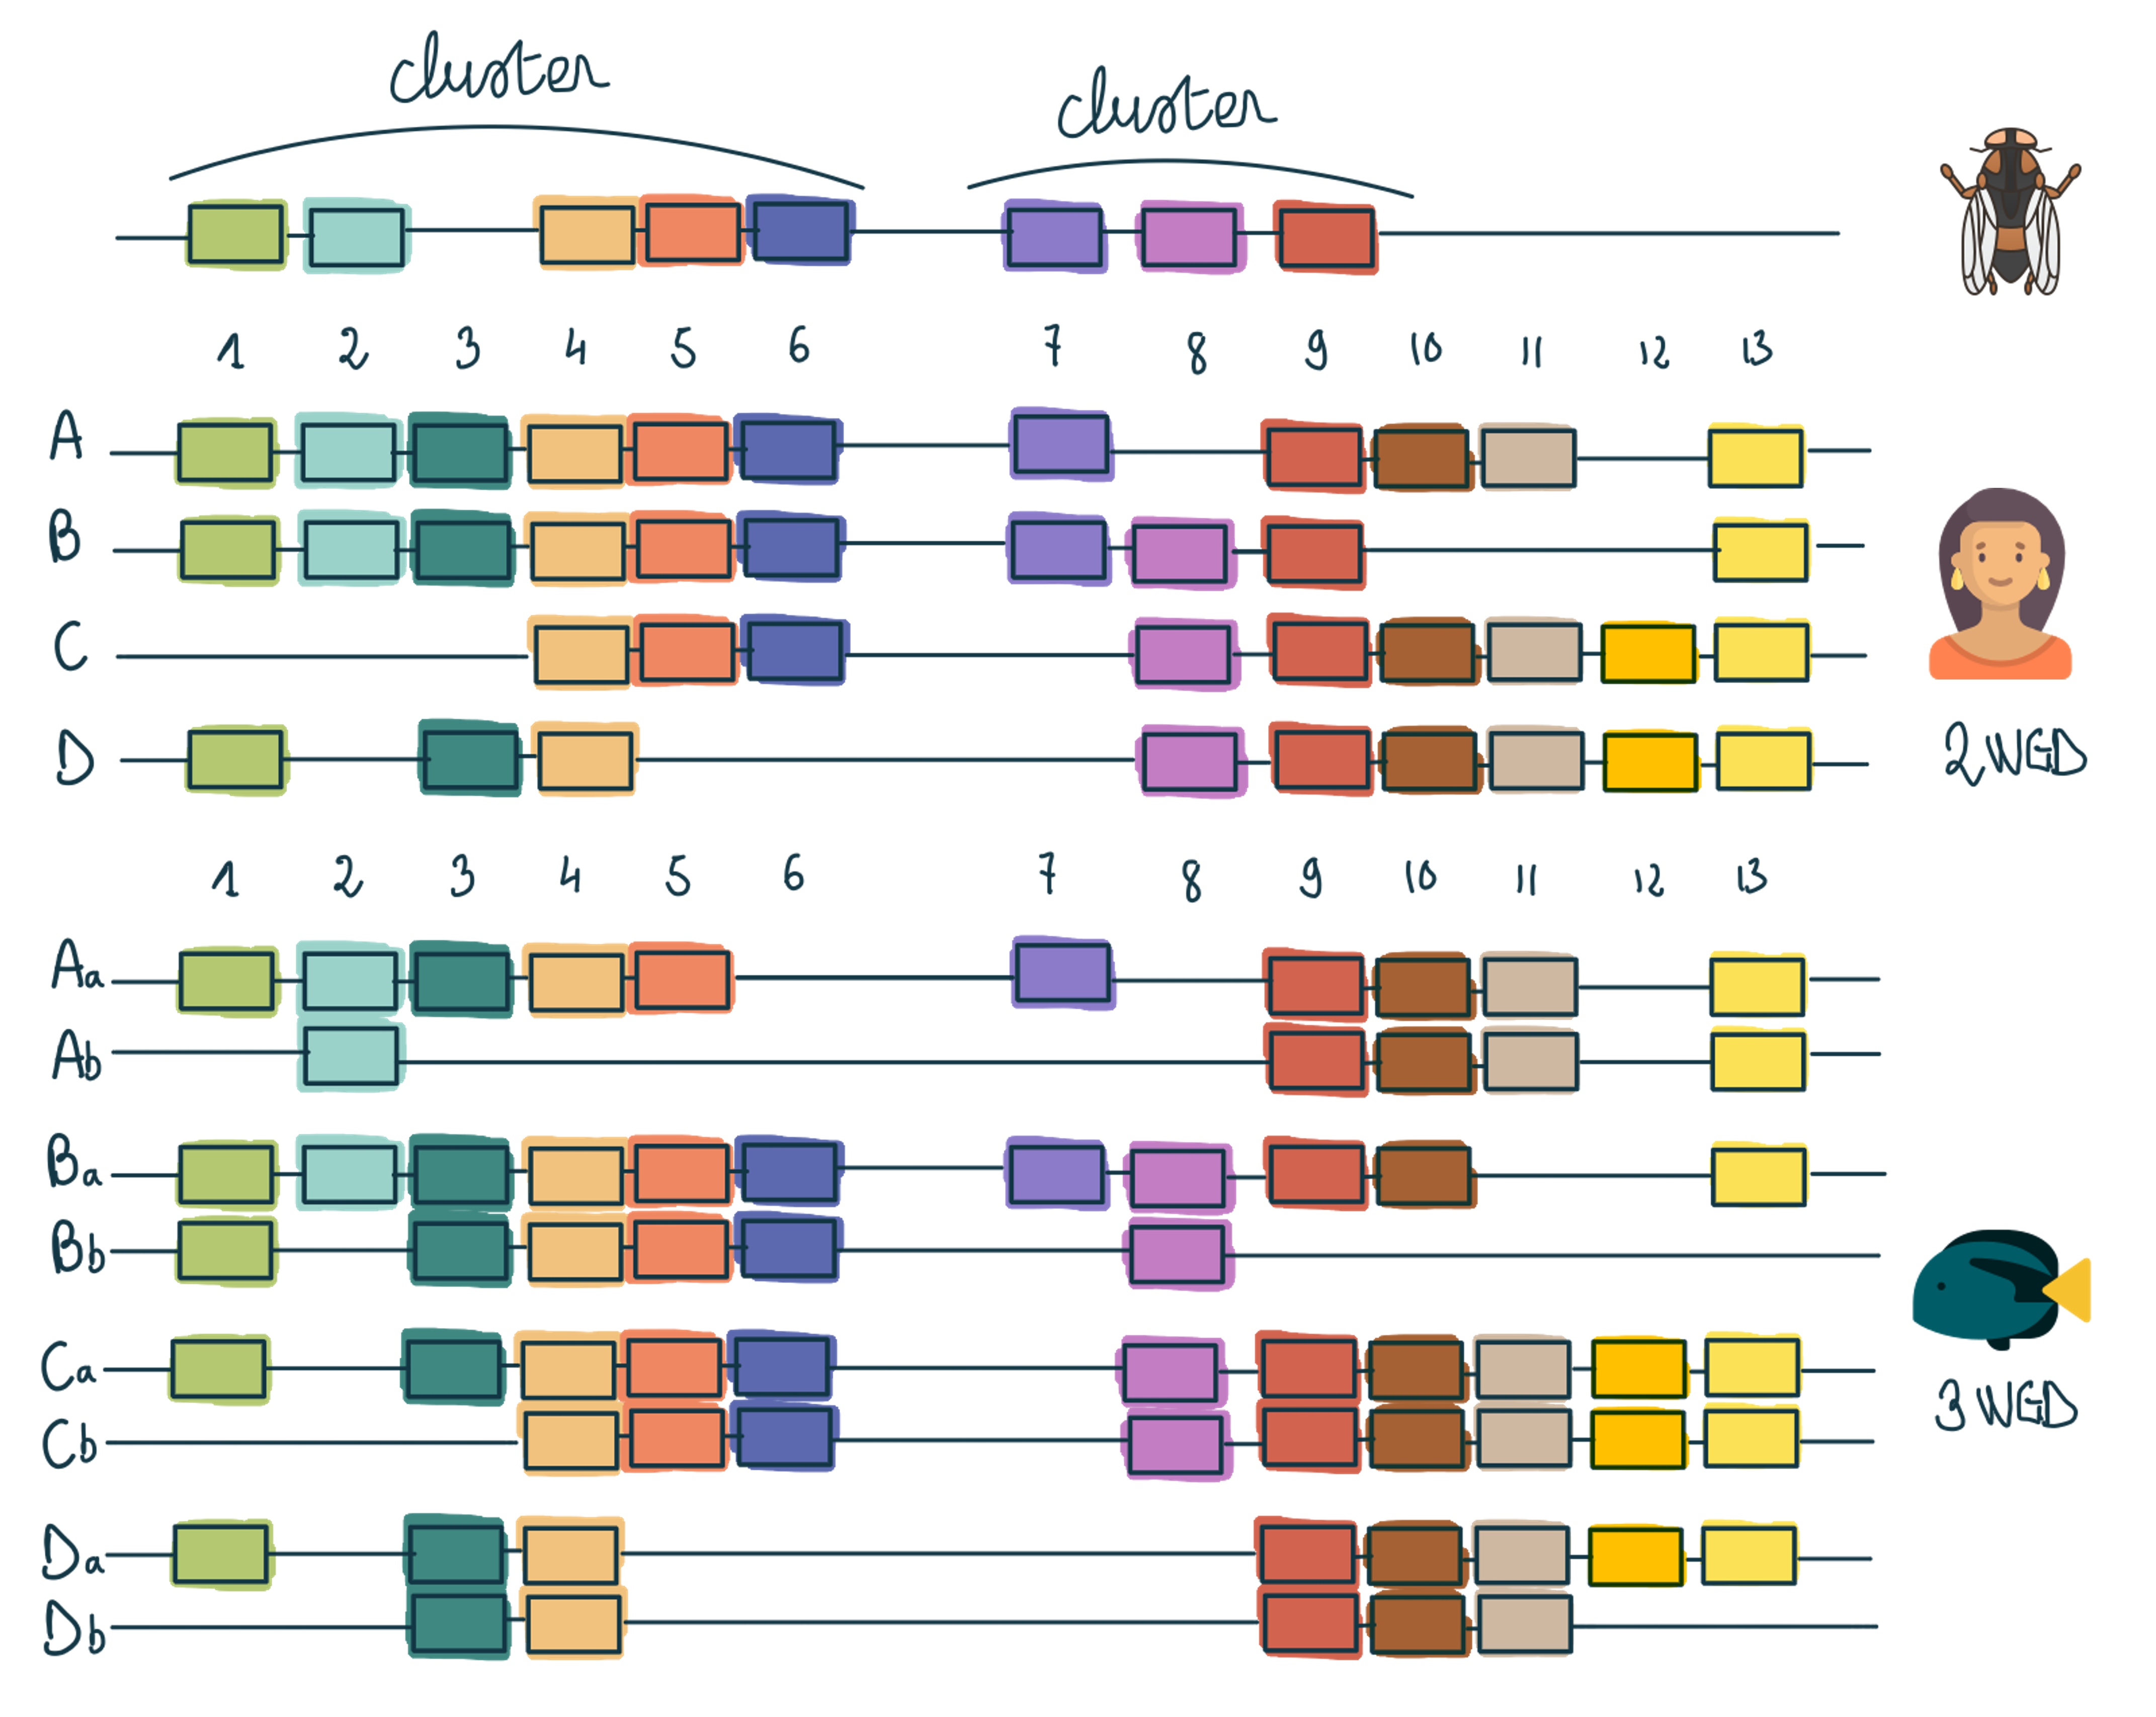
\includegraphics[width=1\textwidth]{figures/corps/figure3.png}
    \caption{Organisation des gènes Hox chez la drosophile, les mammifères et les téléostéens}
    \label{fig:3_hox}
\end{figure}
Légende : Chaque carré représente un gène Hox. Pour la drosophile, les clusters vont de 1 à 6 puis de 7 à 13. Pour les mammifères et les téléostéens, ce seront préférentiellement les différentes lettres A à D. Les gènes partageant la même couleur sont des orthologues. 
Entre la drosophile et les mammifères, le gène 2 s’est subdivisé en 2 et 3, et le gène 9 s’est subdivisé en 9 à 13. Les mammifères qui sont un groupe d’espèces à 2 WGD (duplication de génome complet) comptent environ 39 gènes, et les téléostéens (3 WGD) comptent environ 63 gènes Hox. (Par ailleurs, le cluster Dd des téléostéens n’est pas largement représenté par l’ensemble des téléostéens). Cette figure a été réalisée à partir de plusieurs références \cite{amores_zebrafish_1998, guo_hox_2010, lappin_hox_2006, rux_hox_2017}. \newpage

\par Ces duplications de génomes sont également étudiées pour la recherche médicale. Il a récemment été montré que dans plusieurs cas de tumeurs, des duplications de génome étaient impliquées \parencite{gemble_genetic_2022}. Cette étude montre une forte instabilité génétique après des événements de WGD, ce qui favoriserait les multiples mutations. 
Les duplications de génome sont également connues pour être suivies de perte massive de gènes dupliqués \parencite{inoue_rapid_2015, jaillon_genome_2004}. Ce phénomène, qui est toutefois mal connu, s’appelle la rediploïdisation et consiste en un retour au nombre initial de gènes et non des chromosomes. Pour certains gènes, une seule copie des gènes sera maintenue, ce qui réduit grandement le nombre de paralogues issus de duplication de génome complet \parencite{byrne_yeast_2005}. Par exemple, si le génome de la drosophile partage un patrimoine génétique en commun avec l’homme et compte environ 15 000 gènes codant des protéines, et avec les 2 duplications de génome qu’ont vécu les vertébrés, l’homme devrait avoir environ 60 000 gènes, or, il n’en compte qu’environ 22 000 gènes codants des protéines. Par ailleurs, certains gènes maintenus en duplicat sont responsables de démence chez l’homme, comme la duplication du gène SNCA impliqué dans la maladie de Parkinson \parencite{chartier-harlin_alpha-synuclein_2004, ibanez_causal_2004}. 
La question que nous pouvons nous poser est : quelle force évolutive régit les gènes restés en duplicat ou revenus en singleton ? 

\subsection{Coévolution}\label{coevo}
\par Concernant la force évolutive qui agit sur les gènes, nous n’avons pas de réponse claire et universelle à donner. Cependant, des pistes pourraient expliquer cette pression, comme celle de la coévolution. La coévolution est le fait que des gènes évoluent ensemble en réponse les uns aux autres \parencite{lovell_integrated_2010}. Et c'est ce que Thompson avait défini en 1994 comme étant la coévolution réciproque \parencite{thompson_coevolutionary_1994}. 
\par Un exemple assez parlant est celui des gènes du système immunitaire. Les gènes du système immunitaire n’ont pas d’autres choix que d’évoluer en fonction de l’évolution des pathogènes qui eux-mêmes évoluent en fonction du système immunitaire \parencite{schlesinger_coevolutionary_2014}. 
\par La coévolution est également très étudiée pour les interactions ligands récepteurs, en effet cette interaction est soumise à une certaine pression notamment au niveau de leur site de liaison qui peut être unique en fonction de la spécificité de la relation. Pour le couple OXT-OXTR (l’ocytocine et son récepteur) par exemple, les séquences moléculaires ont longtemps été pensées comme intactes chez les mammifères, seulement, il a été montré quelques différences subtiles qui seraient corrélées avec les changements comportementaux sexuels chez les primates étudiés \parencite{vargas-pinilla_evolutionary_2015}.


\subsection{Naissance et mort des gènes}\label{naissance}
\par Entre les mutations ponctuelles, les duplications de génome, et les pertes massives qui ont suivi, il est question de la naissance et de la mort des gènes. La revue de \cite{kaessmann_origins_2010} détaille les différents types de naissance d’un gène. Nous allons en expliquer quelques-uns. 
\par Dans un premier temps, un nouveau variant d’un gène peut naître d’une mutation ponctuelle. En effet, une mutation peut modifier la séquence nucléotidique d’un gène déjà existant sans qu’il soit pseudogénisé. Un nouveau gène peut apparaître et potentiellement une nouvelle protéine fonctionnelle. 
\par Dans un deuxième temps, la duplication est un moteur clé de la création de nouveaux gènes, que la duplication soit une duplication complète du génome, d’un chromosome uniquement ou même juste localement d’un gène ou d’une partie de séquence. 
\par La naissance des gènes est un mécanisme indispensable à la spéciation et l’adaptation des espèces. Par ailleurs, ce sont des processus très longs, tout comme la mort d’un gène. Si un gène peut naître d’une duplication ou d’une mutation, ce sont les mêmes processus qui peuvent l’amener à la mort. Comme nous l’avons vu dans le Chapitre ~\ref{wgd} page ~\pageref{wgd}, une mutation impliquant un codon stop prématuré peut aboutir à un pseudogène. 
\par Nous pouvons déterminer si un gène est mort en comparant sa séquence à celle d’une autre espèce proche, mais pour laquelle le gène est fonctionnel. À partir de l’alignement de séquence, il est possible de retrouver, comme dans le cas de figure présenté en Figure \ref{fig:4_blast}, une mutation qui remplace un acide aminé par un codon stop (*) par exemple. \newpage

\begin{figure}[H]
    \centering
    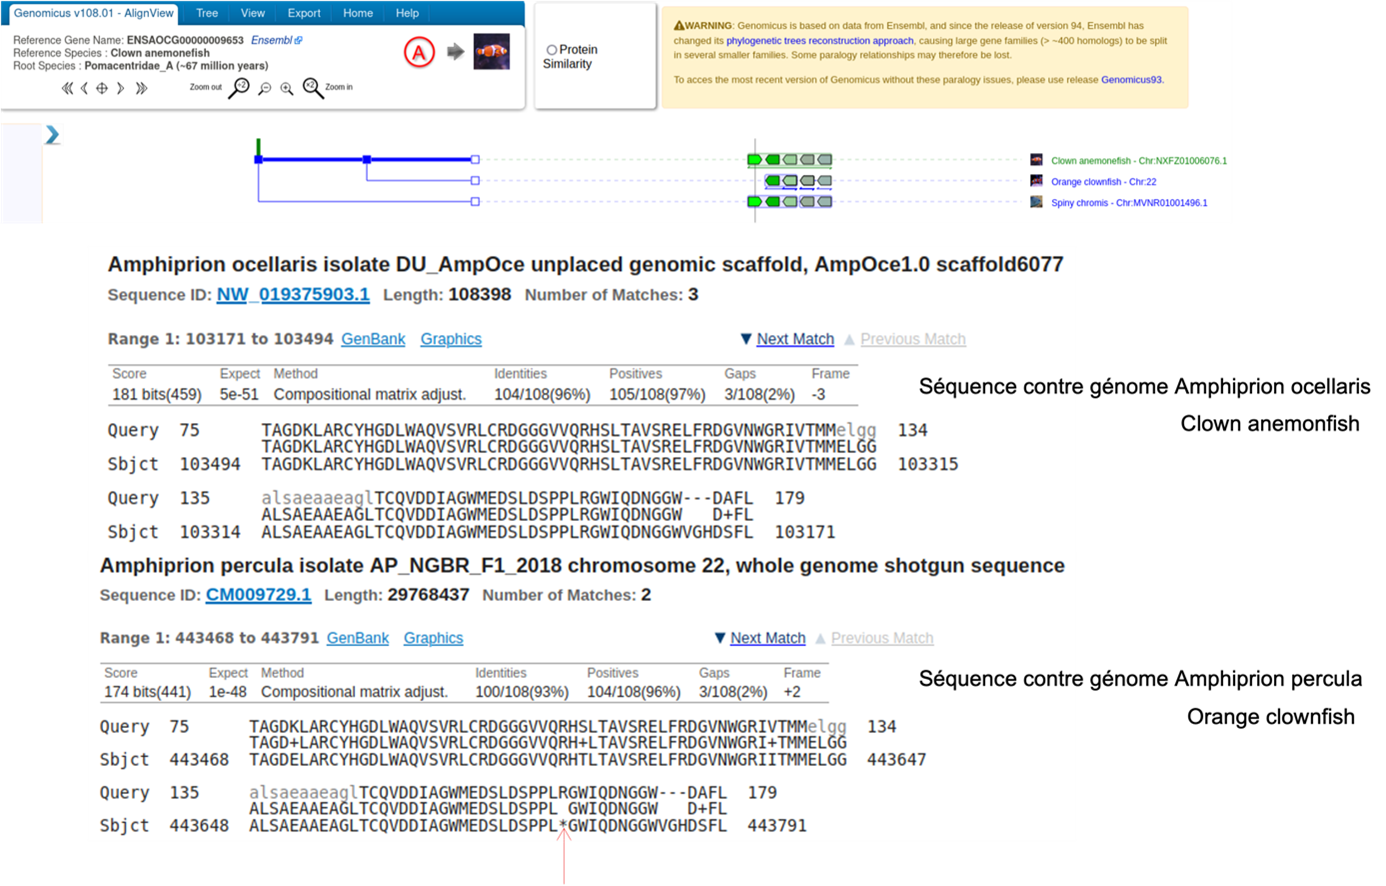
\includegraphics[width=1\textwidth]{figures/corps/figure4.png}
    \caption{Exemple d'un pseudogène avec BLAST}
    \label{fig:4_blast}
\end{figure}
Légende : Dans la première partie de la figure, il s’agit d’une capture d’écran de l’alignement des gènes (synténie, décrit en chapitre \ref{genomicus}), centré sur le gène en vert (ENSAOCG00000009653, BCL2) qui est présent chez les espèces \textit{Clown anemonfish} et \textit{Spiny chromis}, mais absent chez \textit{Orange clownfish}. Il y a donc une suspicion de pseudogène, car la séquence semble être conservée pour les gènes à proximité. Une fois la séquence protéique du gène bcl2 de l’espèce \textit{Clown anemonfish} récupérée, on l’aligne sur son génome. Aucune particularité à observer. Puis, on l’aligne sur l’espèce \textit{Orange clownfish}, et là, on remarque qu’il y a un codon stop (*) qui s’est glissé dans la séquence au niveau de l’Arginine. Le gène est bien pseudogénisé chez cette espèce. 

\newpage
\section{Phylogénie des animaux}\label{phylo}
\par La phylogénie s’est définie graduellement. D’abord avec le Suédois Carl Von Linné au XVIII$\textsuperscript{e}$ siècle qui s’impose avec l’idée de biodiversité et sa classification de plus de 10 000 espèces en binôme genre-espèce. Ce sont ensuite les travaux de Lamark au XIX$\textsuperscript{e}$ siècle qui évoquent les liens de parenté et la transmission du patrimoine génétique d’un parent à ses descendants. Et c’est en 1859 que Charles Darwin publie son ouvrage « De l’origine des espèces » qui soudera la théorie de l’évolution selon laquelle les êtres vivants sont issus d’ancêtres communs, et l’évolution des espèces se produit grâce à la sélection naturelle (caractère héréditaire favorisant la reproduction et la survie de l’espèce). 
\par Avec le temps, les méthodes se sont vues améliorées, nous sommes passés d’une classification morphologique à une classification par la séquence ADN. 


\subsection{Principe de la phylogénie}\label{principephylo}
\par Le principe de phylogénie reprend notamment les travaux de Charles Darwin, et repose principalement sur le fait que chaque organisme descend d’un ancêtre commun. On représente communément les relations de parenté entre les organismes dans un arbre. Les arbres sont constitués de branches qui représentent les liens de parentés, et les nœuds les points de divergence. Ils sont construits à partir d’alignement de séquences et permettent de refléter la proximité entre celles-ci. 
\par Différentes méthodes existent afin de parvenir à représenter l’histoire évolutive des séquences : 
\begin{itemize}
    \item Méthode de parcimonie (la méthode la plus simple, car on considère le minimum d’événement évolutif), 
    \item Méthode de distance (on considère la distance entre les espèces par le nombre de différences entre les séquences), 
    \item Méthode basée sur le maximum de vraisemblance (méthode qui va utiliser les probabilités d’obtention d’un arbre en fonction de plusieurs scénarios), 
    \item ou encore des méthodes plus complexes pour des arbres comportant des hybridations et donc ne peut être définie de manière arborescente \parencite{tagu_bio-informatique_2010}.
\end{itemize}
\par Chaque méthode de reconstruction d’arbre a ses avantages et ses faiblesses, et dépend principalement des données et des objectifs. Cependant, il est préférable de combiner plusieurs méthodes et d’utiliser une méthode d’estimation de la robustesse des nœuds une fois l’arbre généré. La robustesse est estimée par la méthode de \textit{bootstrap} par exemple qui consiste à compter le nombre de fois qu’une branche est présente dans un pool d’arbres échantillons obtenu à partir d’alignements prit aléatoirement dans notre jeu de données.
\par Deux types d’études peuvent être considérés en phylogénie. Dans un premier temps, il y a la phylogénie des espèces, qui place des espèces par rapport à d’autres. Et dans un deuxième temps, il y a la phylogénie des gènes qui permet de mettre en relation des similitudes des gènes. Les arbres de gènes peuvent être différents des arbres des espèces. Pour exemple, le gène FOXP2, aussi appelé le « gène de la parole » est présent chez des espèces vertébrées comme l’homme, la souris, la chauve-souris ou encore des oiseaux \parencite{enard_molecular_2002, scharff_evolutionary_2005, webb_foxp2_2005, white_singing_2006}. La séquence protéique est fortement conservée chez toutes les espèces, à l’exception de la chauve-souris qui pourrait être liée à l’écholocalisation chez celle-ci \parencite{li_accelerated_2007}. En représentant l’arbre du gène FOXP2 et l’arbre des espèces, on se rend compte qu’ils ne sont pas identiques ou congruents (Figure \ref{fig:5_foxp2}). 
\par Dans notre cas, nous avons travaillé avec des arbres phylogénétiques de gènes et certains concepts et termes sont à définir, comme l’homologie, l’orthologie et la paralogie.

\begin{figure}[H]
    \centering
    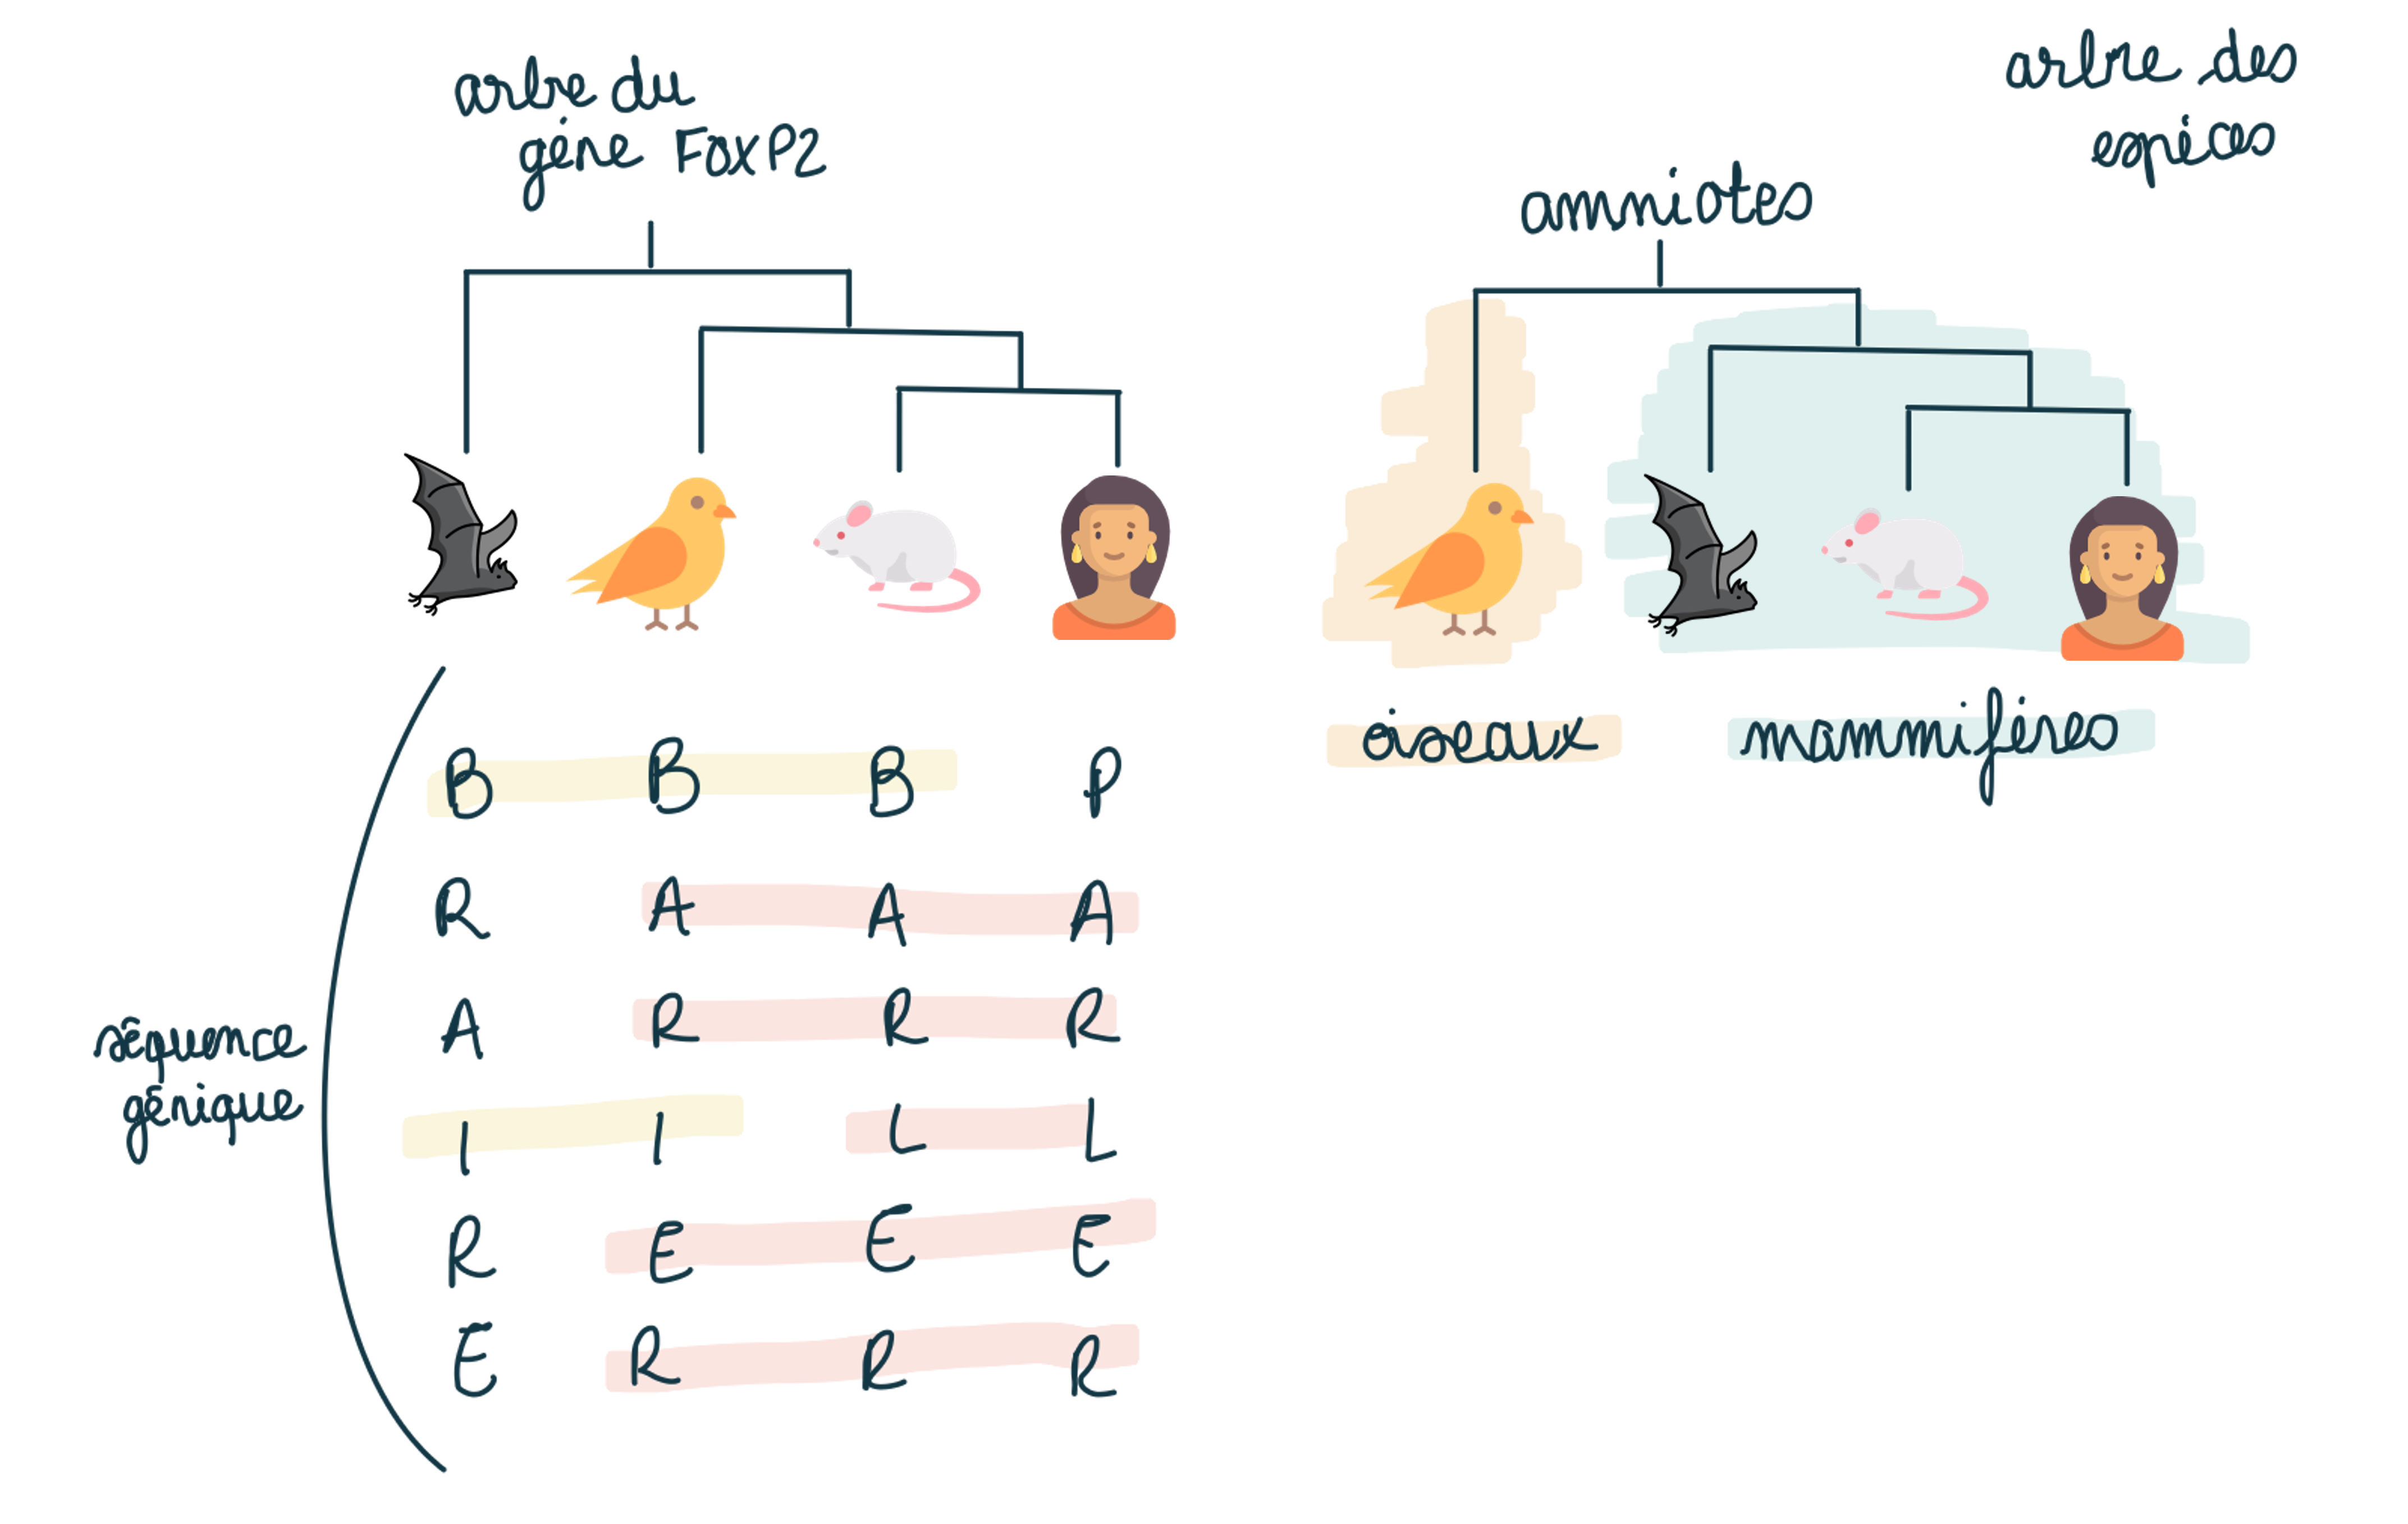
\includegraphics[width=1\textwidth]{figures/corps/figure5.png}
    \caption{Différences entre arbre de gènes et d'espèces}
    \label{fig:5_foxp2}
\end{figure}
Légende : À gauche, il y a l’arbre du gène FOXP2 en fonction de l’alignement des différentes séquences. À droite, il y a l’arbre des espèces. \newpage

\subsection{Homologie, orthologie et paralogie}\label{homologie}
\par Homologie, orthologie et paralogie désignent tous les 3 des degrés différents d’évolution de parcours des gènes. 
\par Le terme homologie se réfère aux similitudes de séquences entre plusieurs gènes, il englobe les termes paralogie et orthologie. Deux gènes ayant un ancêtre commun sont dits « homologues ».
\par La paralogie fait référence à des gènes issus d’une même descendance, mais ayant subi des duplications génétiques au sein d’une même espèce. Ils peuvent avoir subi également des mutations qui ne les rendent pas identiques. De plus, les gènes paralogues n’ont pas forcément la même fonction, il est même plutôt fréquent d’avoir une néo-fonctionnalisation (nouvelle fonction du gène), une sous-fonctionnalisation (les deux gènes acquièrent une sous-fonction de la fonction mère du gène), une spécialisation spatio-temporelle ou une spécialisation de fonction \parencite{kuzmin_retention_2022}.
\par L’orthologie concerne les gènes partageant un ancêtre commun suivi d’un événement de spéciation, donc d’espèces différentes \parencite{fitch_distinguishing_1970}. La définition d’un orthologue est simple lorsqu’on parle de deux gènes, mais se complique rapidement lorsqu’on parle de plusieurs gènes pour plusieurs espèces. Et pourtant, c’est bien grâce aux relations d’orthologie que l’on a fait des avancées en génomique comparative et pour l’annotation des nouveaux génomes séquencés \parencite{huerta-cepas_fast_2017}. 
\par Les relations d’homologies sont donc étroitement liées les unes avec les autres et peuvent être complexes. Au sein des arbres phylogénétiques, il y a à la fois, les orthologues et les paralogues. Pour être plus précis, lorsque des orthologues n’ont pas subi de duplication par la suite, ils sont appelés orthologues directs. Le terme paralogue direct existe également pour les gènes dupliqués au sein d’une même espèce. (Figure \ref{fig:6_ortho}). 
\par Les gènes paralogues issus de duplication de génome sont appelés onhologue en mémoire à Ohno qui a mis en lumière les duplications de génome chez les vertébrés \parencite{ohno_evolution_1968}. Les gènes ohnologues représentent entre 20 et 35\% des gènes humains et concernent majoritairement les gènes de transduction du signal (74\%) \parencite{singh_identification_2015}. 
\par De plus, il existe également des catégories pour parler du nombre d’orthologues du gène chez deux espèces. Premièrement, nous avons l’orthologie un à un (1:1), qui correspond à un orthologue strict chez une espèce d’un gène chez une autre espèce. Ensuite il y a les co-orthologues qui peuvent être un-à-plusieurs ou plusieurs-à-un (1:n), qui comme son nom l’indique évoque un exemplaire d’un gène chez une espèce, et plusieurs dans une autre. Puis les orthologues plusieurs-à-plusieurs (m;n), ainsi que les orthologies complexes prenant en compte les pertes de gènes, les duplications de génomes et autres évènements d’évolutions complexes (Figure \ref{fig:5_foxp2}) \parencite{koonin_orthologs_2005}.

\begin{figure}[H]
    \centering
    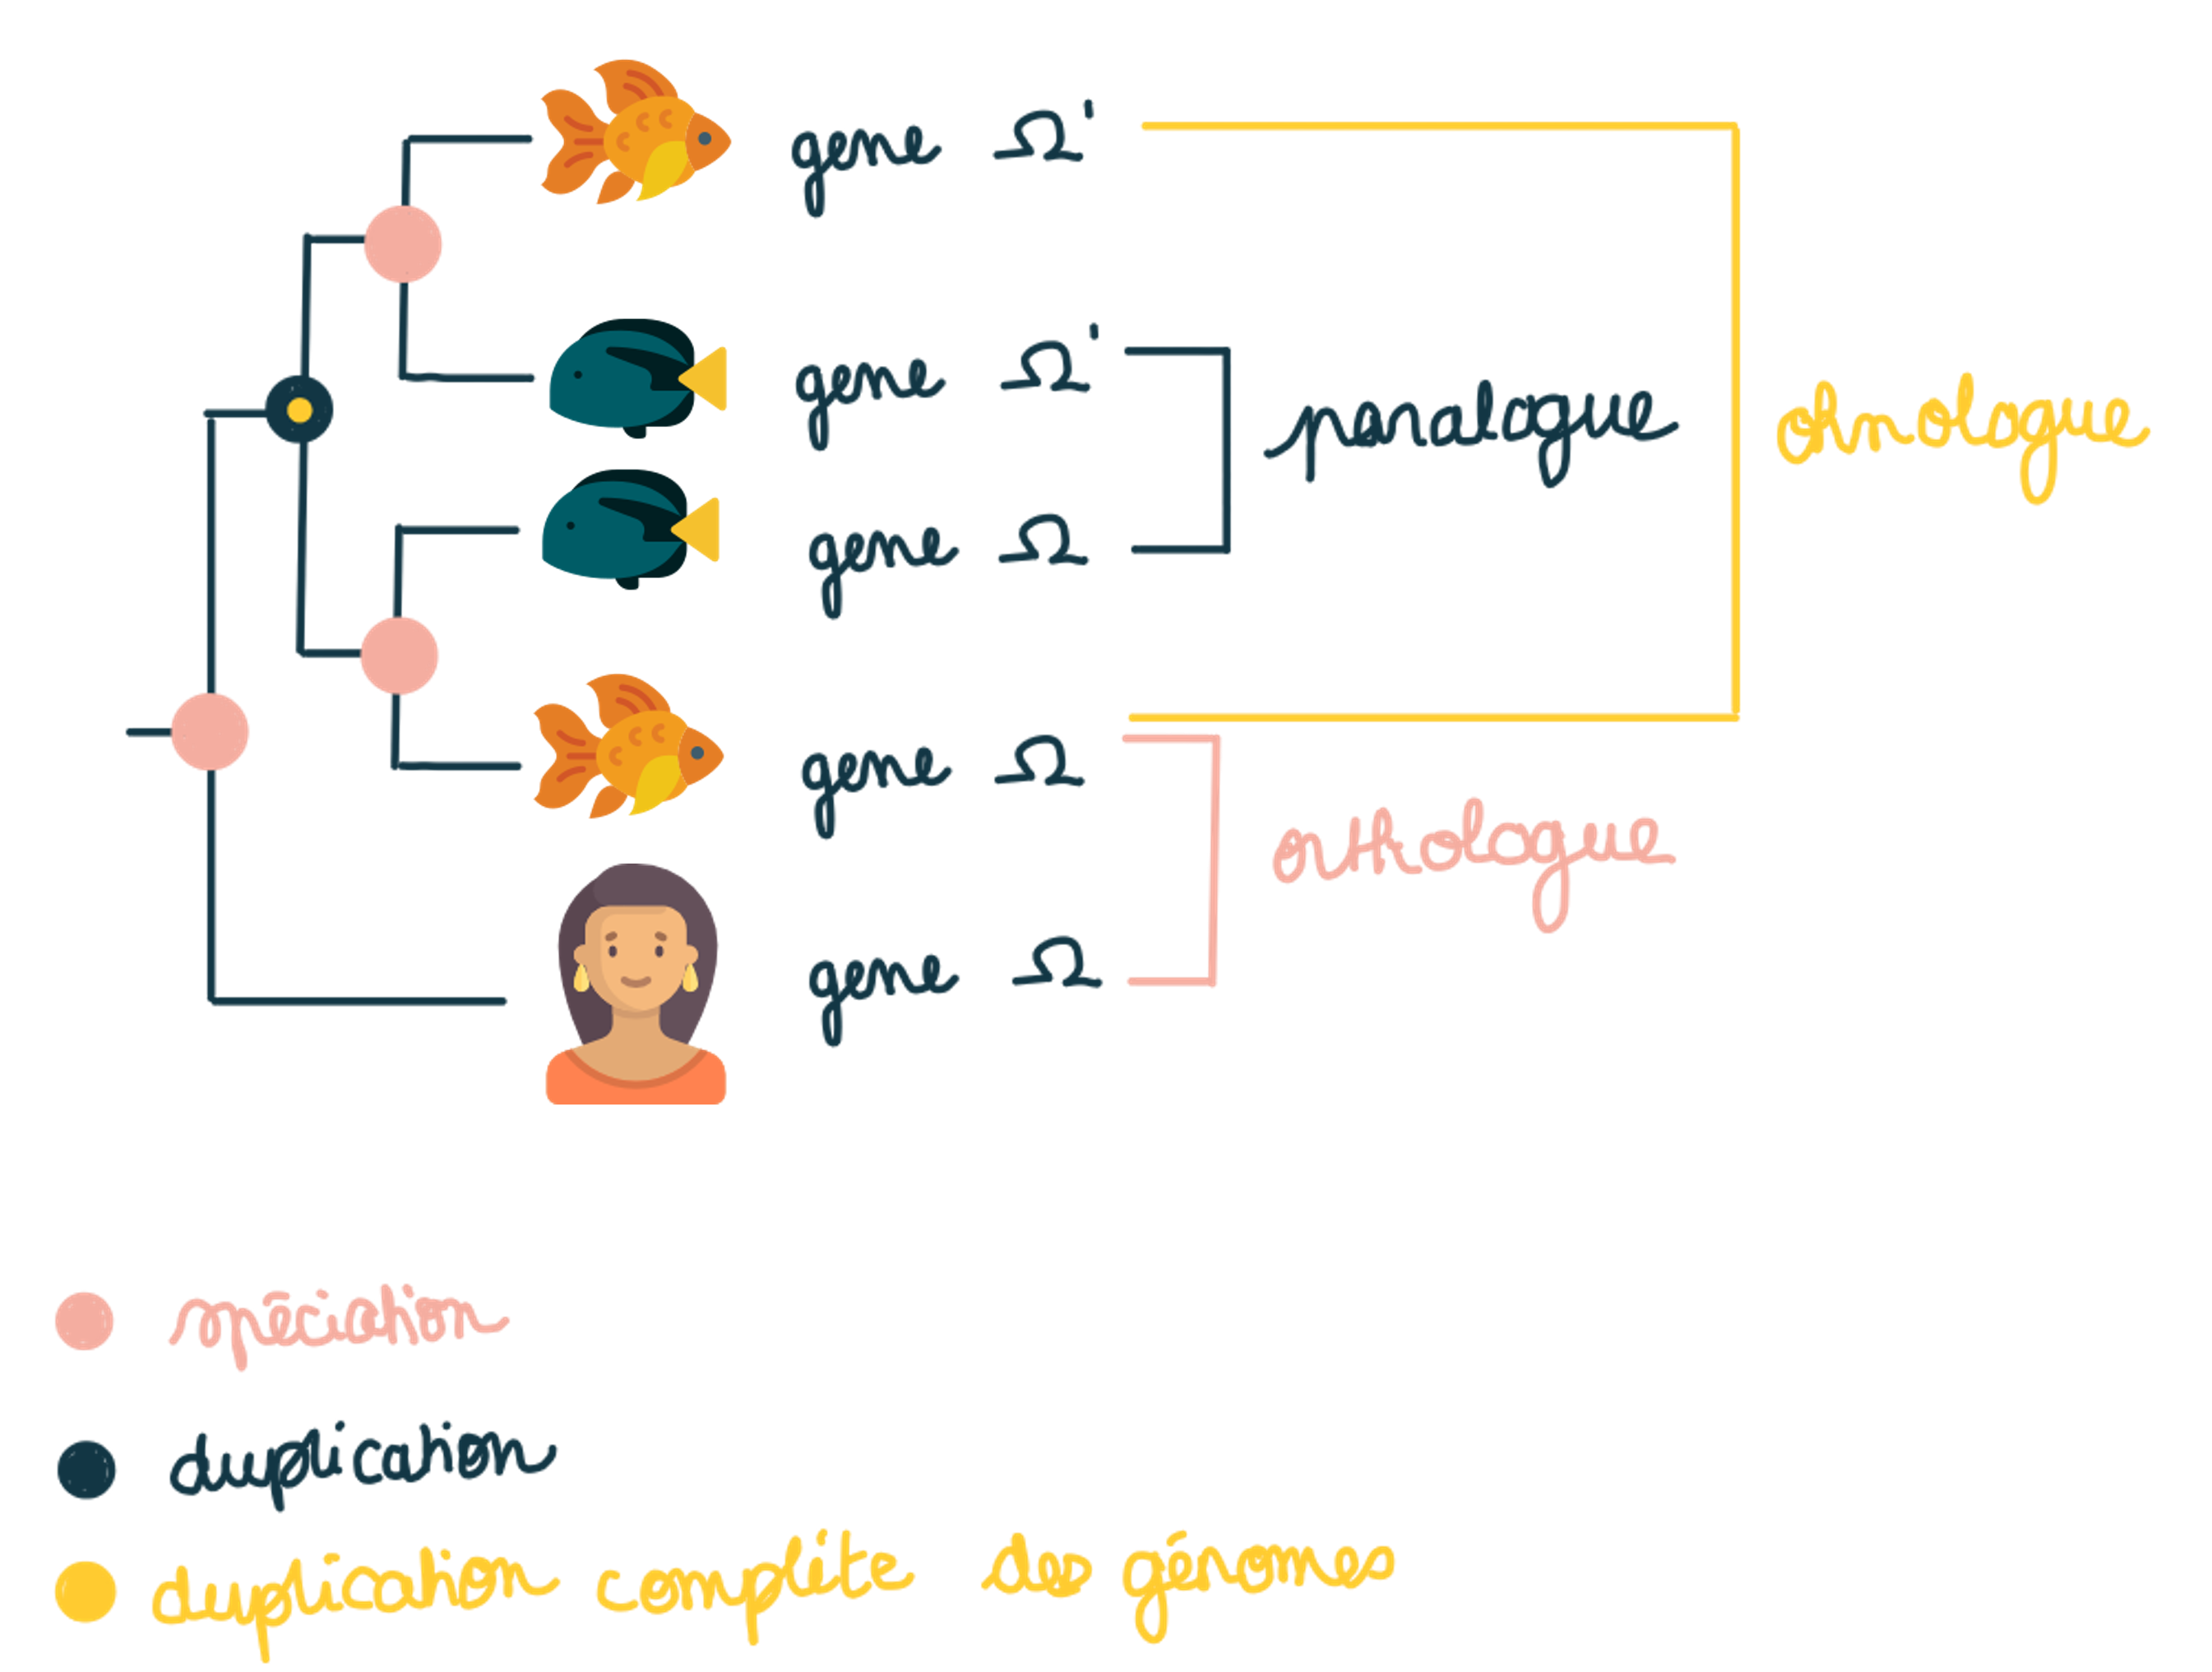
\includegraphics[width=1\textwidth]{figures/corps/figure6.png}
    \caption{Représentation des différents homologues}
    \label{fig:6_ortho}
\end{figure}
Légende : En rose sont représentés les orthologues à la suite d’une spéciation. En noir, les paralogues à la suite d’un évènement de duplication et en jaune les gènes ohnologues à la suite d’une duplication complète des génomes. 

\subsection{Arbre de la vie des animaux}\label{tree}
\par Comme évoqué dans le chapitre précédent, les relations entre les espèces peuvent être représentées en arbre, appelé « arbre des espèces ». Ces arbres renferment la proximité des espèces (proximité des branches), leur temps de divergence (longueur des branches) ainsi les évènements vécus au fil du temps (nœud) avec comme exemple les duplications de génome entre autres. Les arbres phylogénétiques utilisent également des termes de la classification taxonomique des espèces. 
Mais, il existe des biais à l’élaboration d’un arbre de la vie comme la convergence évolutive. La convergence évolutive est le mécanisme par lequel des espèces n’ayant pas d’ancêtre commun proche évoluent dans la même direction. En d’autres termes, elles n’ont pas reçu de caractère commun de leur descendance commune, mais l’ont acquis indépendamment l’une de l’autre. En génomique, la convergence évolutive se traduit par une mutation similaire dans des gènes spécifiques distincts. Ça peut être le cas notamment pour les résistances aux bactéries. Cela peut donc devenir un biais dans le sens où des évènements de mutations semblables ayant lieu après divergence des espèces peuvent rapprocher ces deux espèces dans l’arbre de la vie par erreur \parencite{christin_causes_2010}. Il a été montré que les systèmes olfactifs des vertébrés et celui des protostomiens partagent des arrangements physiologique similaires \parencite{hildebrand_mechanisms_1997} mais diverses origines \parencite{strausfeld_olfactory_1999}.
\par Dans notre cas, nous utilisons à tort le terme « arbre de la vie des animaux » car nous étudions l’ensemble du règne animal ainsi qu’une espèce du règne des champignons (*Saccharomyces cerevisiae*). L’ensemble des deux règnes est nommé Opisthoconte (\textit{Opisthokonta}) (Figure \ref{fig:7_arbre}). 
\par Dans notre étude, nous avons dû partir de l’homme, car c’est l’espèce la plus référencée, et la plus étudiée au niveau des voies de signalisation, comme nous le verrons par la suite. De ce fait, l’utilisation du terme « remonter l’arbre » sera utilisé à l’avenir car on remonte les branches de l’arbre à partir de l’homme pour aller vers ses ancêtres communs avec d’autres espèces sur le chemin. 
\par Plus nous parcourons l’arbre vers l’ancêtre commun le plus éloigné, et moins nous aurons de similitude avec les différentes espèces. Au sein de l’espèce, nous partageons notre génome à 99,9\%, c’est ce 0,01\% qui explique nos différences comme la couleur de nos cheveux, la couleur de nos yeux, notre taille ou nos allergies. Nous partageons 98,7\% de notre patrimoine génétique avec le chimpanzé, 90\% avec le chat domestique, 85\% avec la souris, et plus étonnant, 26\% avec la levure et 18\% avec les champignons de Paris \parencite{roy_biotechnology_2010}. Ces valeurs sont déterminées en utilisant uniquement les gènes codants. Or, les gènes codants ne représentent que 5\% du génome humain. Et par complémentarité, le génome humain est constitué à 6\% de gènes communs à l’ensemble des primates, 13\% aux vertébrés, 16\% aux animaux, 28\% aux eucaryotes et 37\% aux bactéries \parencite{domazet-loso_ancient_2008, mcfall-ngai_animals_2013}.
\par De connaître ces similitudes a permis de connaître et comprendre l’arbre de la vie dans son entièreté. C’est tout particulièrement important dans notre étude, car nous allons remonter l’arbre de la vie des Opisthocontes (Figure \ref{fig:8_opistho}), pour connaitre l’origine des gènes impliqués dans une voie de signalisation. Cet arbre simplifié des différents nœuds et clades est notre point de repère pour la première étude. Un nombre de 25 clades a été sélectionné pour définir nos moments d’apparitions. L'estimation du moment où un gène est apparu se base sur l'observation de son orthologue le plus éloigné dans l'arbre phylogénétique, c'est-à-dire le point ancestral le plus éloigné où un orthologue du gène humain peut être identifié. Pour illustrer, si un gène humain possède un orthologue chez les poissons, mais que cette homologie ne se poursuit pas au-delà, on peut supposer que le moment de l'apparition de ce gène remonte probablement au nœud des \textit{Eutelostomi}.

\begin{figure}[H]
    \centering
    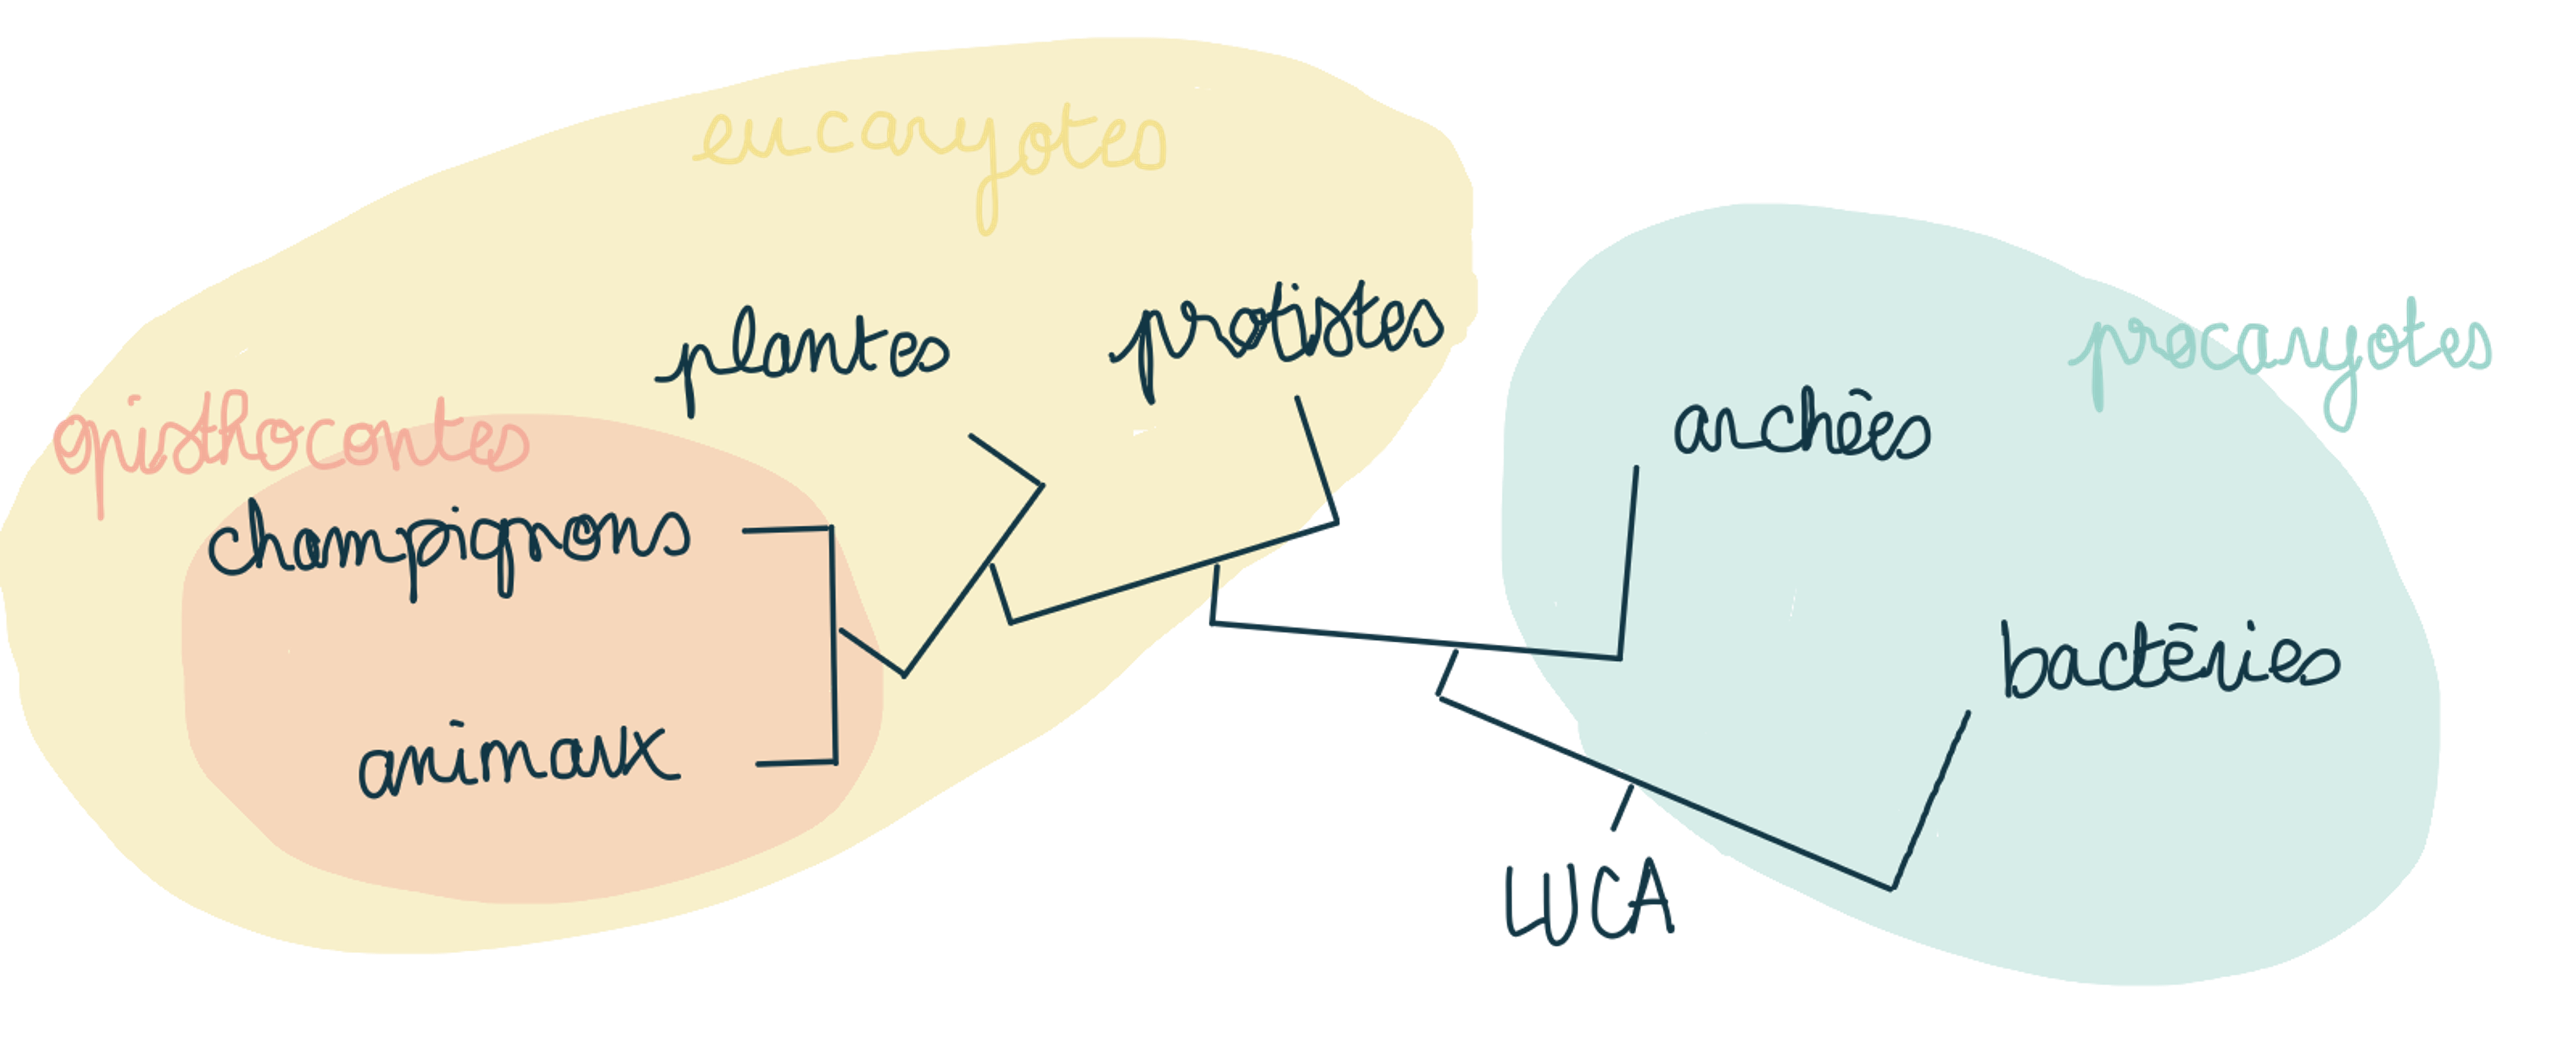
\includegraphics[width=0.7\textwidth]{figures/corps/figure7.png}
    \caption{Arbre de la vie}
    \label{fig:7_arbre}
\end{figure}
Légende : LUCA pour Last Universal Common Ancestor, en français le Dernier ancêtre commun universel. \\
\begin{figure}[H]
    \centering
    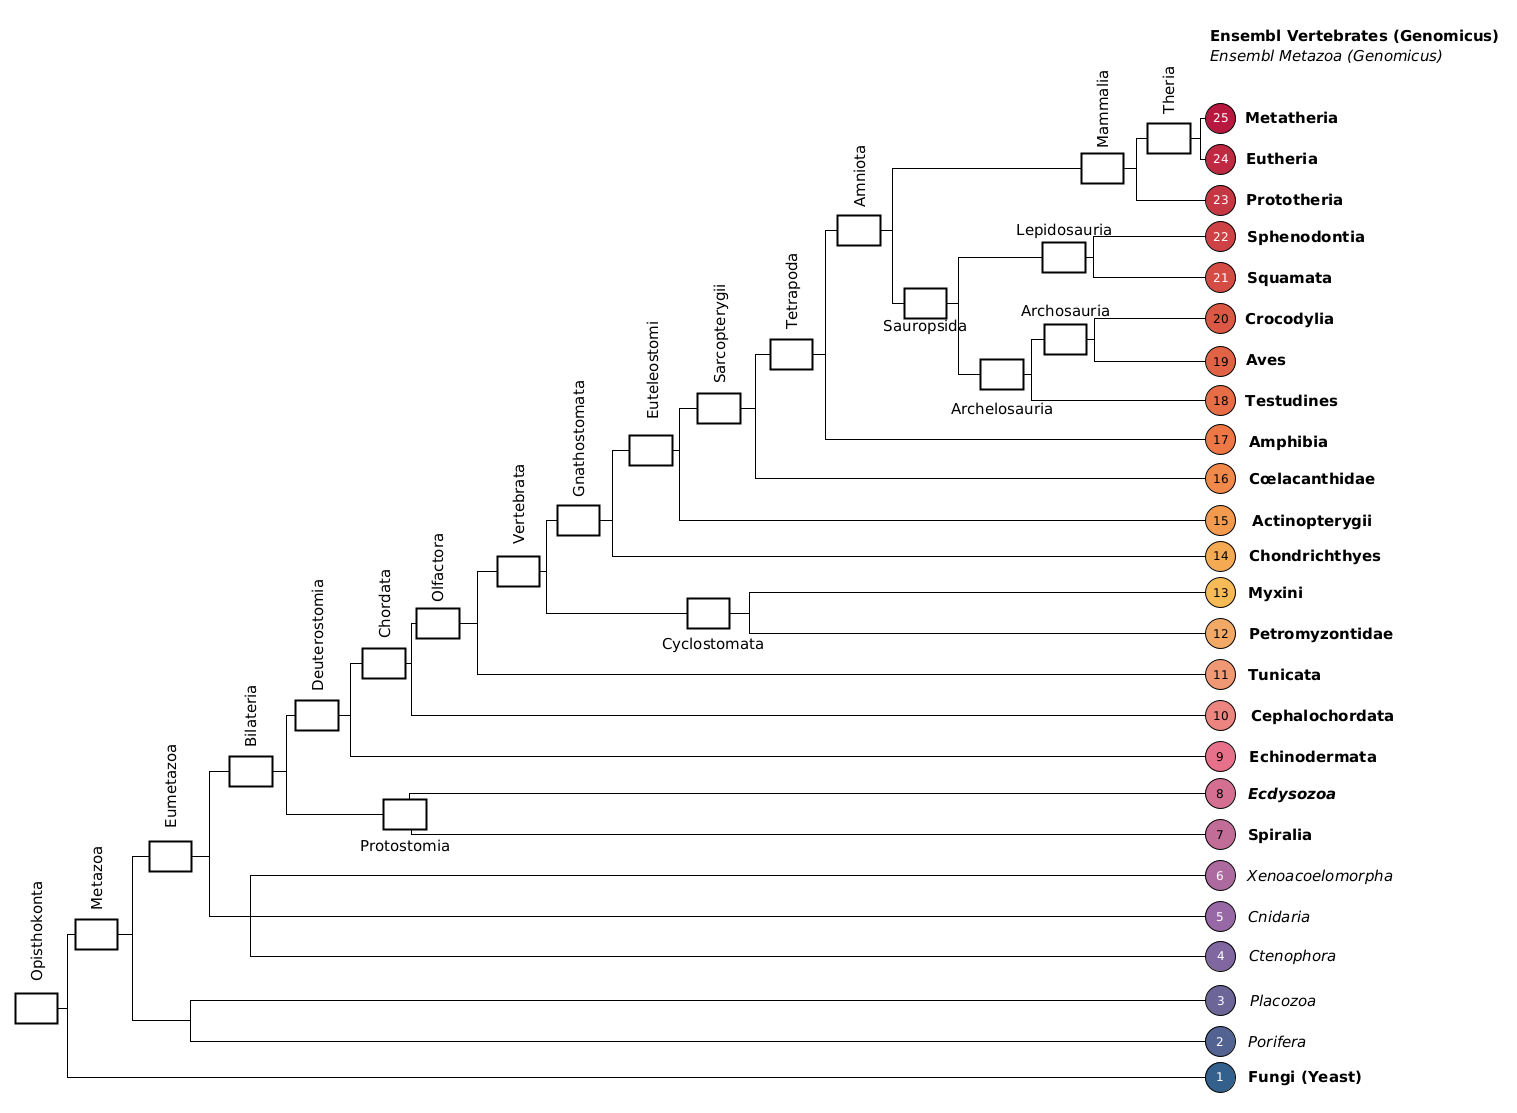
\includegraphics[width=1\textwidth]{figures/corps/figure8.png}
    \caption{Arbre de la vie des Opisthocontes simplifié pour notre étude}
    \label{fig:8_opistho}
\end{figure}
Légende : Chaque rectangle représente un nœud de spéciation au cours de l’évolution. Chaque branche représente un clade terminal de l’arbre avec son numéro associé dans les ronds de couleurs. La longueur des branches n’est pas représentative de la divergence évolutive réelle. En gras sont les clades disponibles sur Genomicus Vertebrates, et en italique les clades disponibles sur Genomicus Metazoa. \newpage

\subsection{Spécificité des téléostéens}\label{teleost}
\par Un clade parmi les animaux va nous intéresser particulièrement pour l’étude 2, il s’agit des poissons téléostéens (\textit{Teleostei}). Les téléostéens font partie du sous-embranchement des vertébrés, qu'ils représentent largement, car approximativement 50\% des vertébrés sont des téléostéens. Environ 25 000 espèces composent ce clade, et la diversité de ce groupe permet difficilement une définition globale. Cependant, ils se caractérisent par leur ossature complète, ils ont des nageoires rayonnées, et une mâchoire. Ce qui exclut les poissons cartilagineux comme les raies et les requins. D’un point de vue morphologique et écologique, les téléostéens sont très diversifiés. Certains peuvent vivre en eaux douces ou en eaux salées, en eaux profondes et pour quelques-uns avoir des interactions avec le monde terrestre. Ils peuvent également avoir des stratégies de reproduction variées (ovipare, vivipare et même ovovivipare). 
\par Cette diversité pourrait être due à la troisième duplication de génome complet partagée par l’ensemble des espèces de téléostéens en plus des deux survenues pour l’ensemble des vertébrés \parencite{ravi_rapidly_2008, taylor_genome_2003}. Par ailleurs, les téléostéens ne dérogent pas à la règle et leur troisième duplication de génome est également suivie d’une période de rediploïdisation (perte massive de gènes dupliqués) \parencite{inoue_rapid_2015}. 
\par Une troisième duplication est donc spécifique aux téléostéens, mais à cela s’ajoute une quatrième duplication pour deux clades distincts des téléostéens : les salmonidés et les carpes \parencite{jaillon_genome_2004, lien_atlantic_2016}  (Figure \ref{fig:9_teleosts}).
\par La découverte de cette troisième duplication de gènes a pour origine l’identification de 7 complexes Hox en 1998 chez le poisson zèbre contre 4 chez l’homme \parencite{amores_zebrafish_1998} tandis qu’on en trouvera 8 chez le \textit{Japanese eel} qui est également un téléostéen \parencite{guo_hox_2010} (Figure \ref{fig:3_hox}). \newpage

\begin{figure}[H]
    \centering
    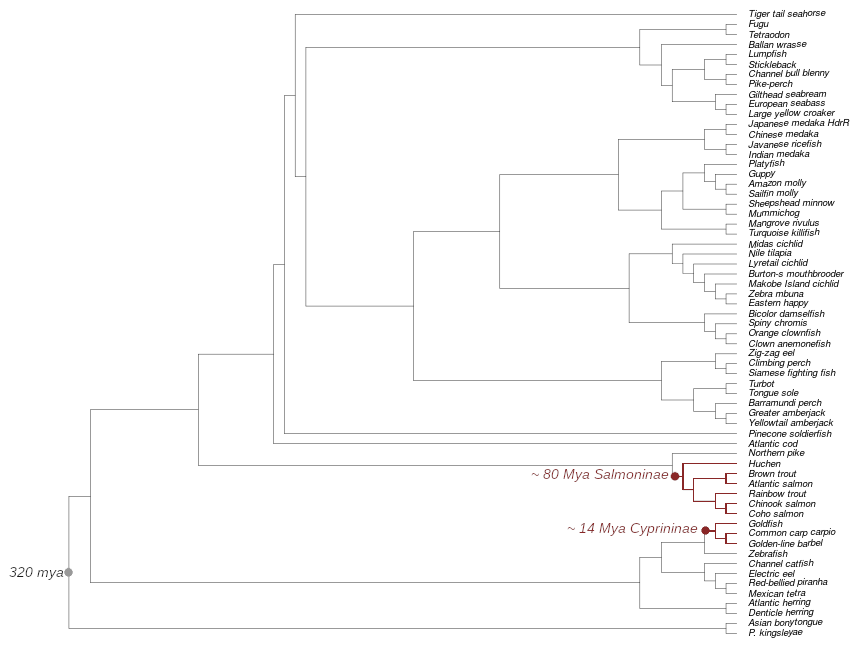
\includegraphics[width=1\textwidth]{figures/corps/figure9.png}
    \caption{Arbre des téléostéens}
    \label{fig:9_teleosts}
\end{figure}
Légende : Les nœuds avec un point correspondent au moment de duplication de génome. Les branches noires sont les espèces 3 WGD, et en rouge les espèces 4 WGD. \\

\subsection{Bases de données}\label{bdd}
\par Durant cette étude, nous avons utilisé différentes bases de données mettent à disposition des arbres phylogénétiques, comme notamment la base de données Ensembl, ainsi que la base de données Genomicus. Genomicus est basée sur les données d’Ensembl, et les deux bases de données existent pour différents règnes : \textit{Vertebrates, Bacteria, Fungi, Plants, Protistes et Metazoa}. Dans les deux sous-chapitres suivants, nous décrierons le fonctionnement général pour Vertebrates, mais ils fonctionnent tous de la même façon. 


\subsubsection{Ensembl}\label{ensembl}
\par Premièrement, il est important de présenter la base de données Ensembl \href{https://www.ensembl.org/}{(https://www\\.ensembl.org/)}. Il s’agit d’une base de données regroupant de nombreuses ressources génomiques. Elle offre une annotation complète des gènes, permet de réaliser des alignements de séquences et calcule les alignements multiples. Nous avons utilisé différentes versions de la base de données. Chaque version étant la plus récente au moment des études. La dernière version que nous avons utilisée est la version V109. Elle comprend 199 espèces de vertébrés. Dans notre cas, nous avons utilisé Ensembl BioMart notamment pour l’étude 2. BioMart est un outil d’Ensembl permettant des requêtes complexes et automatisées au sein de la base de données comme la recherche d’orthologue par exemple, ou de paralogues, de pourcentages d’homologie (Figure \ref{fig:10_biomart}). 
\par Pour cette étude, nous l’avons utilisé afin de récupérer l’ensemble des orthologues téléostéens des gènes humains codant des protéines. En version 107, il y avait 63 espèces de téléostéens, dont 54 espèces 3 WGD et 9 espèces 4 WGD (Figure \ref{fig:9_teleosts}).

\subsubsection{Genomicus}\label{genomicus}
\par Genomicus \href{https://www.genomicus.bio.ens.psl.eu/}{(https://www.genomicus.bio.ens.psl.eu/)} est une base de données « fille » de la base de données Ensembl car elle utilise les arbres Ensembl pour ses propres outils. Cependant, les arbres Ensembl sont modifiés pour résoudre les problèmes de noeuds de duplications mal documentées. La structure de l'arbre est alors révisée en transformant ces nœuds de duplications mal établis en nœuds de spéciation, tout en réaffectant les quelques gènes dupliqués vers des nœuds plus récents \parencite{louis_genomicus_2015}.
\par Ces arbres sont accessibles au format .nhx (New Hampshire eXtended, format basé sur New Hampshire eXtended, format standard pour les arbres phylogénétique). 
\par Genomicus propose également une visualisation de la synténie des gènes sur les chromosomes, ce qui aura des avantages lors de la recherche de pseudogènes. Le terme synténie vient de la conservation plus ou moins grande de l’ordre des gènes sur un chromosome, relativement entre eux au sein des génomes. (Figure \ref{fig:11_genomicus}). La notion de synténie découle de l’étude comparative des génomes. C’est notamment grâce à cette synténie que nous pouvons différencier les duplications complètes de génome des duplications ponctuelles comme ça a été l’exemple avec la famille des gènes Hox (Figure \ref{fig:3_hox}). \newpage

\begin{figure}[H]
    \centering
    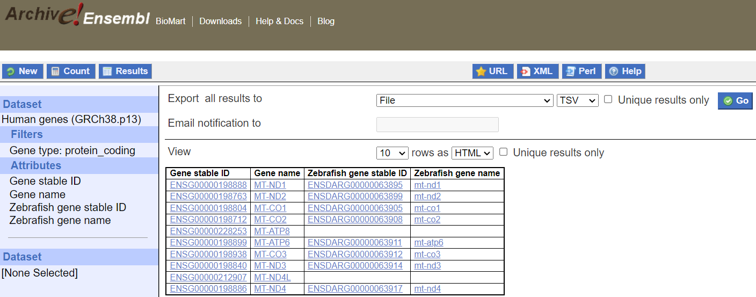
\includegraphics[width=1\textwidth]{figures/corps/figure10.png}
    \caption{Affichage des résultats Ensembl Biomart}
    \label{fig:10_biomart}
\end{figure}
Légende : Dans cet exemple, nous avons effectué la recherche sur la version Ensembl Biomart V107 des orthologues \textit{Zebrafish} de gènes codant des protéines humaines.  \\
\begin{figure}[H]
    \centering
    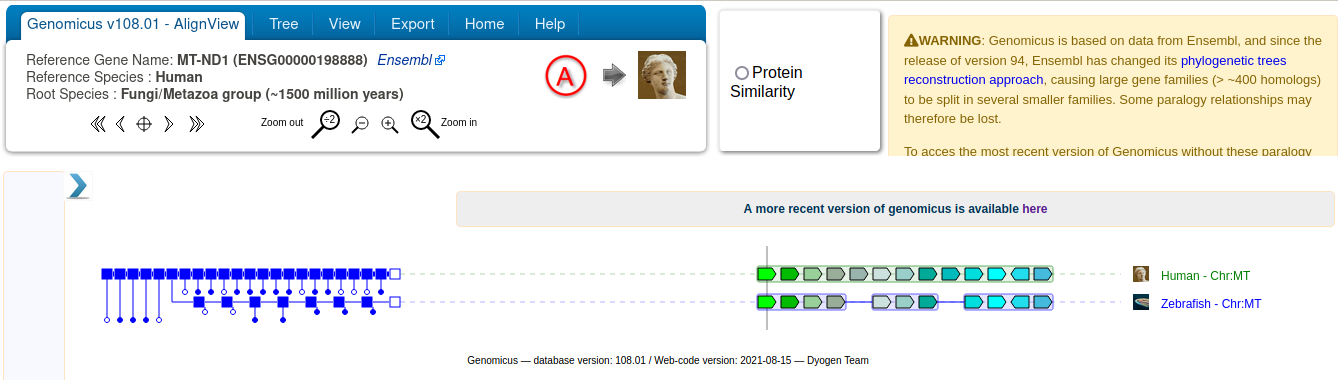
\includegraphics[width=1\textwidth]{figures/corps/figure11.png}
    \caption{Affichage des résultats Genomicus}
    \label{fig:11_genomicus}
\end{figure}
Légende : À partir des résultats Ensembl Biomart, on a été regarder la synténie du gène MT-ND1 entre l’Homme et le \textit{Zebrafish}. Le gène MT-ND1 est coloré en vert. On peut voir que la synténie de cette zone est conservée à l’exception de deux gènes perdus chez \textit{Zebrafish}.

\newpage
\section{Communication cellulaire} \label{commcel}
\par Les voies de signalisation sont un moyen de transmission d’informations pour et par les cellules. Par ce biais, elles permettent le développement, la croissance, le maintien homéostatique des cellules d’organismes multicellulaires \parencite{combarnous_communications_2013}. Les voies de signalisations se caractérisent par une cascade d’interactions protéiques au sein d’une cellule (Figure \ref{fig:12_signa}). Cette cascade est initiée par un ligand se fixant à son récepteur ou en réponse à un \textit{stimuli}, et se terminant par une réponse cellulaire ou la régulation d’un gène. Il existe plusieurs grandes catégories de voie de signalisation qui sont elles-mêmes caractérisées par le type du récepteur. 
\par L’étude des voies de signalisation est nécessaire, notamment pour en apprendre plus sur le fonctionnement des maladies ou les dysfonctionnements entre interactions protéiques. Les études sur les interactions au sein des cellules s’appellent l’interactome. 

\subsection{Interactions protéiques} \label{intprot}
\par Lorsqu’on parle d’interactions protéiques, on peut rapidement parler de biologie systémique car elle fait écho aux études de réseaux complexes d’un organisme. Les protéines interagissent entre elles, mais ne font généralement pas intervenir toute la molécule. Les interactions se font entre des sites de liaison. Les protéines peuvent donc se lier soit spécifiquement avec une protéine partenaire unique, mais peuvent également se lier avec plusieurs partenaires. Ces spécificités d’interactions peuvent être des interactions spécifiques à différentes échelles, au sein d’une cellule, au sein d’un organisme, et même plus largement commune à plusieurs organismes. Dans le cas des interactions multiples, on parle alors d’un site de liaison qui est peu spécifique, et/ou d’une protéine avec plusieurs sites de liaisons \parencite{di_lullo_mapping_2002}. Les interactions peuvent être directes, mais peuvent également se faire à distance grâce à des forces permettant la liaison entre acides aminés : 
\begin{itemize}
    \item Les liaisons électrostatiques et ioniques qui se produisent entre charges opposées,
    \item Les liaisons hydrophobes qui se produisent lorsque les régions hydrophobes des protéines s’attirent, 
    \item Les liaisons hydrogènes se forment lorsque l'atome d'hydrogène est partagé entre deux atomes, l'un étant plus électronégatif que l'autre  \parencite{bondar_hydrogen_2012},
    \item Les liaisons par ponts hydrogènes entre protéines et molécules, 
    \item Les liaisons de Van Der Waals qui se produisent entre atomes non polaires \parencite{van_oss_role_1986}.
\end{itemize}
\par Toutes ces formes différentes de liaisons permettent un panel d’interactions possibles entre les protéines. En multipliant les possibilités d’interactions, on peut s’imaginer qu’elles n’ont pas besoin d’être maintenues dans le temps puisqu’elles trouveront d’une façon ou d’une autre un partenaire avec qui interagir au sein d’une espèce. En 2006, une étude a montré que parmi 70 000 interactions protéine-protéine, seulement 16 étaient communes aux 4 espèces étudiées (vers, mouche, levure et homme) \parencite{gandhi_analysis_2006}. 

\begin{figure}[H]
    \centering
    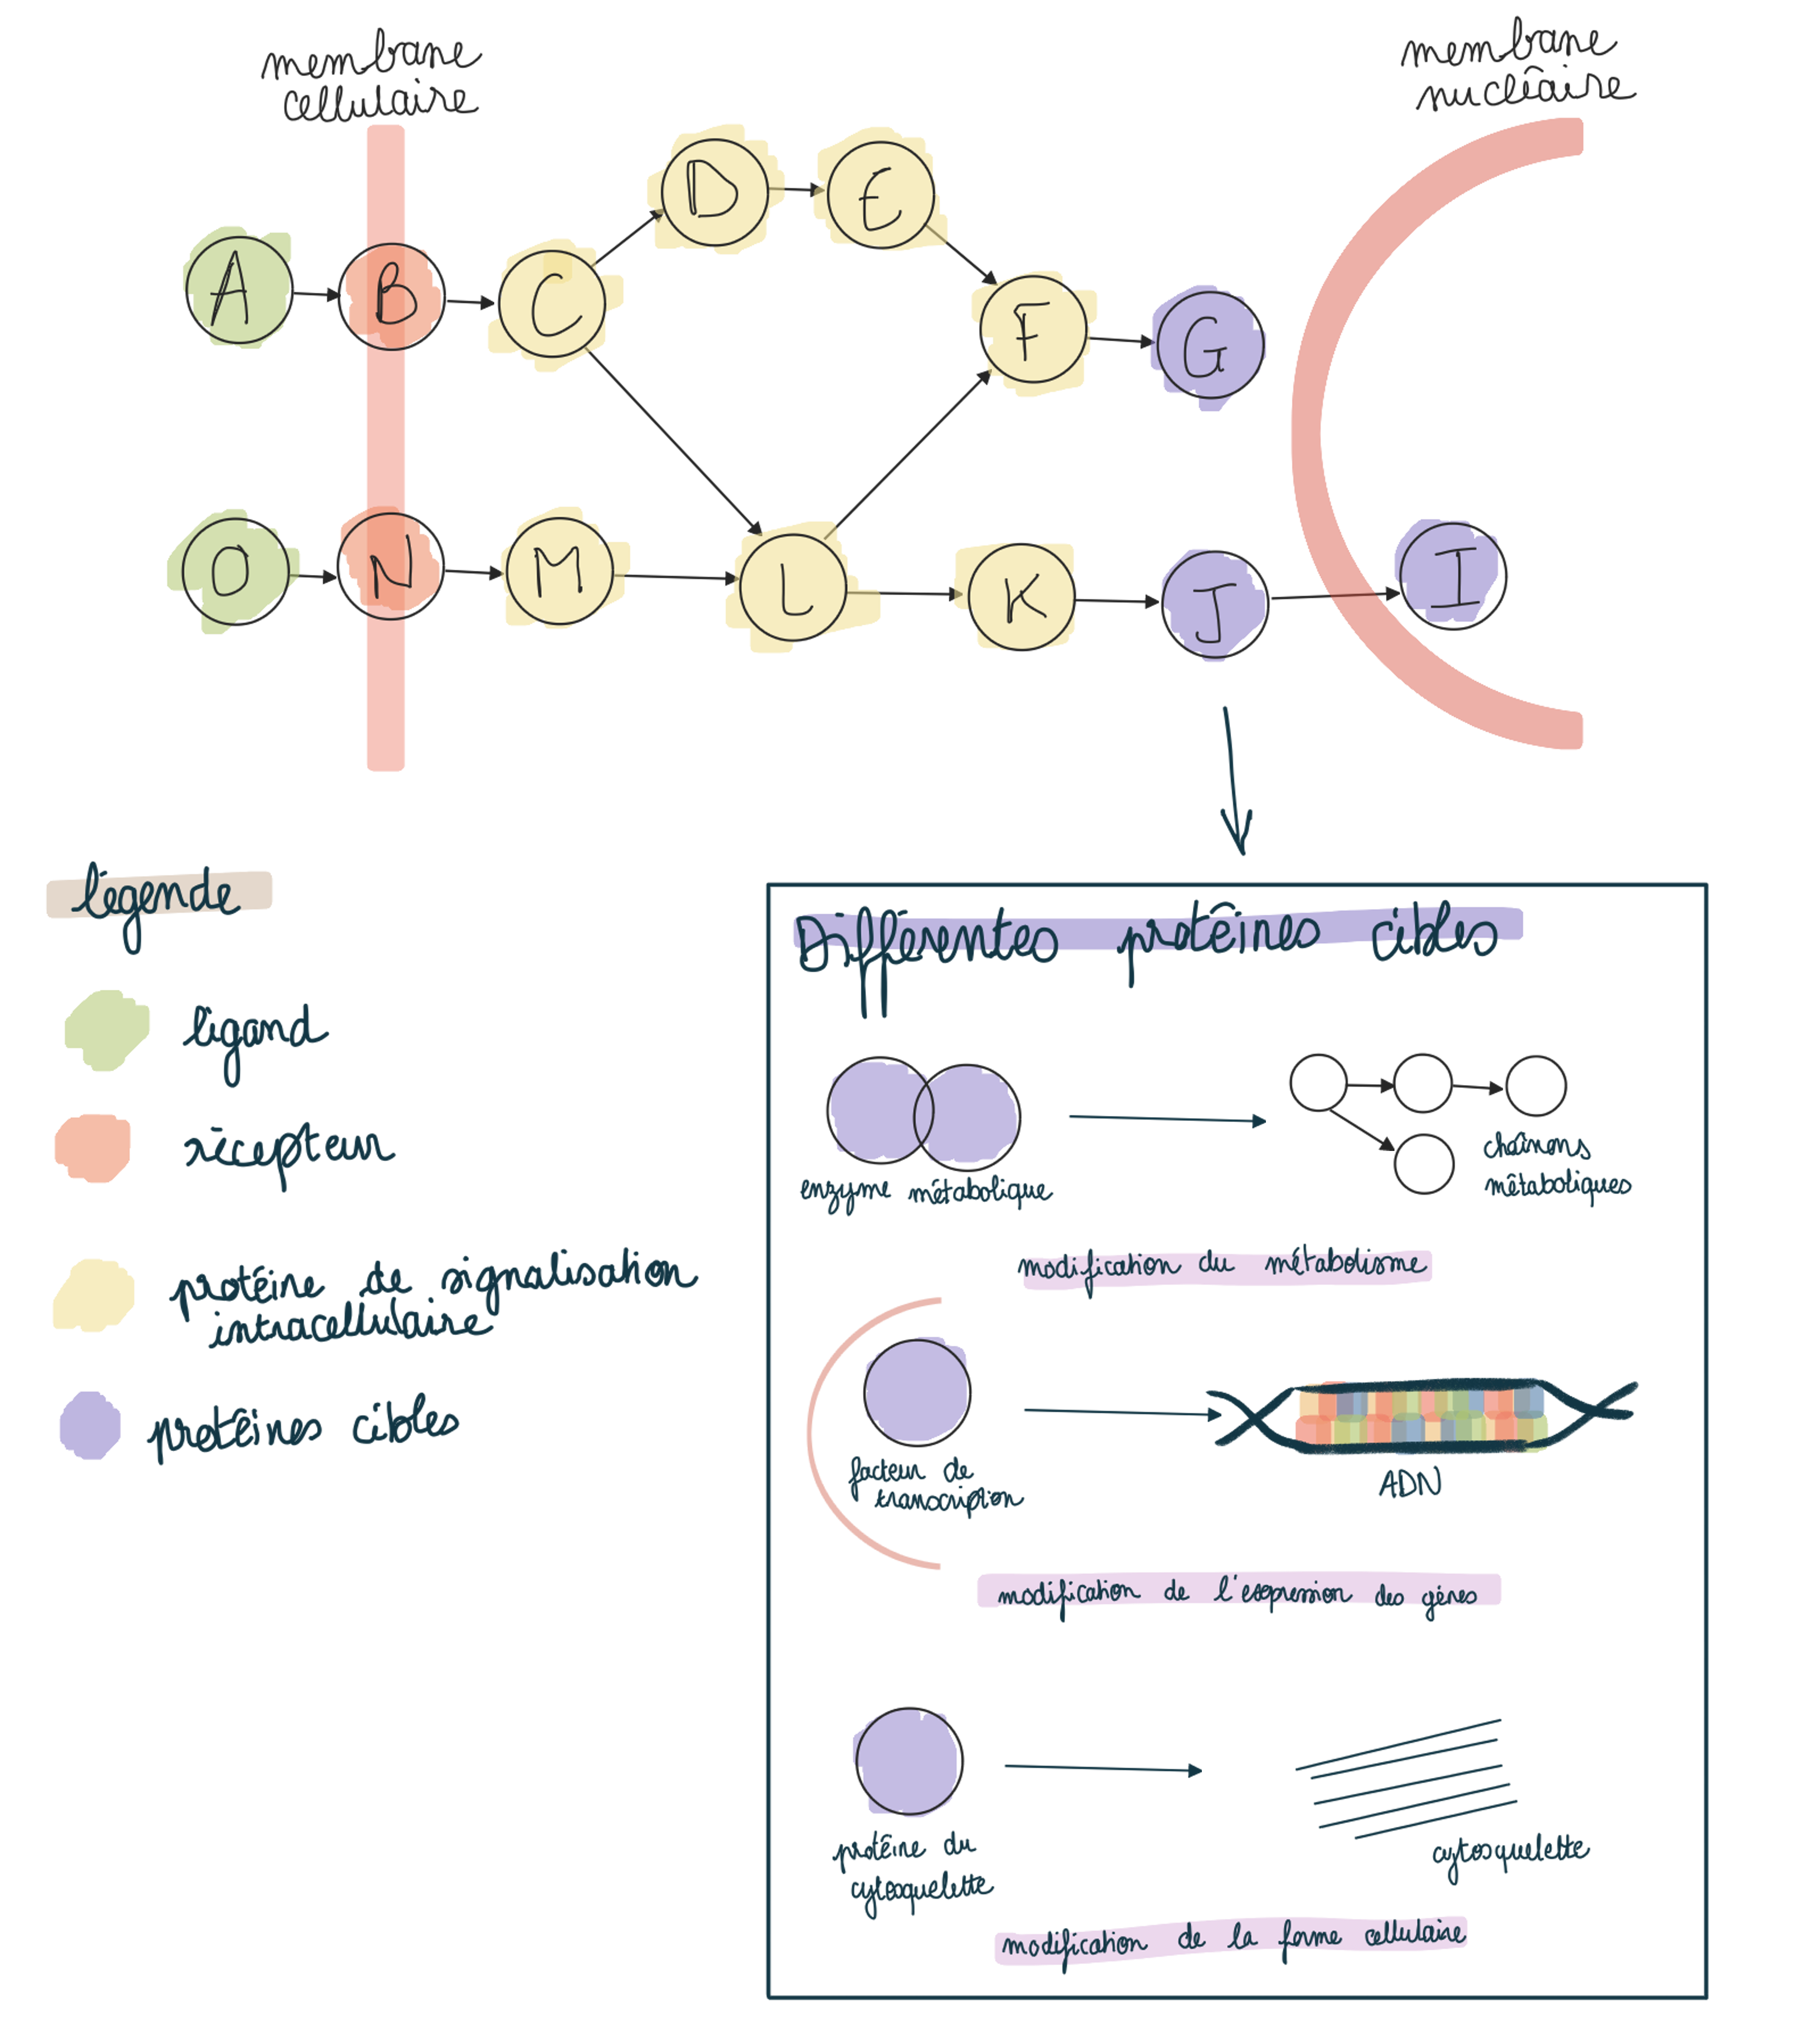
\includegraphics[width=1\textwidth]{figures/corps/figure12.png}
    \caption{Schéma d'une voie de signalisation intracellulaire}
    \label{fig:12_signa}
\end{figure}
Légende : Chaque rond représente une protéine et chaque flèche une interaction.  \newpage

\subsection{Relation ligand-récepteur}\label{ligrec}
\par Les ligands et les récepteurs membranaires sont deux protéines interagissant ensemble au niveau de la membrane d’une cellule. Le ligand se fixant à son récepteur va entraîner l’activation des molécules de la voie de signalisation intracellulaire (Figure \ref{fig:12_signa}).
\par Les relations ligand-récepteur peuvent être, comme toute interaction, soit spécifique, soit non spécifique. Par exemple, la voie JAK-STAT compte environ 60 ligands et 40 récepteurs connus \parencite{darnell_jak-stat_1994}. À l’inverse, la voie de l’insuline est très spécifique de 3 ligands et 2 récepteurs connus \parencite{leroith_insulin-like_2021}. Pour vulgariser les relations ligand-récepteur, on parle très souvent de clé (ligand) et serrure (récepteur). Une clé peut ouvrir plusieurs serrures, et une serrure peut être ouverte par plusieurs clés, mais les deux ont généralement besoin l’un de l’autre pour fonctionner. 
\par De nombreuses études portent sur la coévolution des interactions ligand-récepteur notamment pour des questions médicales, notamment car les médicaments ciblent généralement les récepteurs \parencite{de_jong_receptor-ligand_2005, pluder_proteome_2006, woolhouse_biological_2002}. 

\subsection{KEGG}\label{kegg}
\par Concernant les interactions et les voies de signalisation, il a fallu trouver une source de données nous permettant d’avoir accès à ces informations. Et la base de données KEGG (Kyoto Encyclopedia of Genes and Genome) \href{https://www.genome.jp/kegg}{(https://www.genome.jp/kegg)} est l’une des premières à représenter exhaustivement les interactions au sein d’une cellule sous forme de voies \parencite{bader_pathguide_2006} et une des plus complètes avec 568 voies de signalisation décrites manuellement dont 335 voies humaines \parencite{chanumolu_kegg2net_2021}.
\par La base de données a plusieurs fonctions comme la visualisation d’une multitude de voies, mais également la coloration des gènes au sein des voies. Sur KEGG, les voies sont représentées chez l’homme, et quelques fois pour la levure, la drosophile ou encore plusieurs espèces à la fois. 
\par Elle permet également de récupérer les voies dans un format utilisables par des bibliothèques R. Chaque voie de signalisation a donc été récupérée au format .xml (Extensible Markup Language) à partir de l'outil PATHWAY de KEGG. Ce format de fichier est bien pris en charge par les bibliothèques R telles que XML \parencite{lang_xml_2023} et igraph \parencite{csardi_igraph_2023, csardi_igraph_2006} (Figure \ref{fig:13_kegg}).
\par Pour les deux études, nous avons utilisé la base de données KEGG V104.0. À partir des mots de clés « \textit{signaling pathway} » et « \textit{human} », nous avons récupéré un ensemble de 47 voies de signalisation représentant 2 298 gènes uniques. L’ensemble des voies sont représentées ainsi que leurs caractéristiques dans le Tableau \ref{table:voiecaracteristiq}. 


\begin{figure}[H]
    \centering
    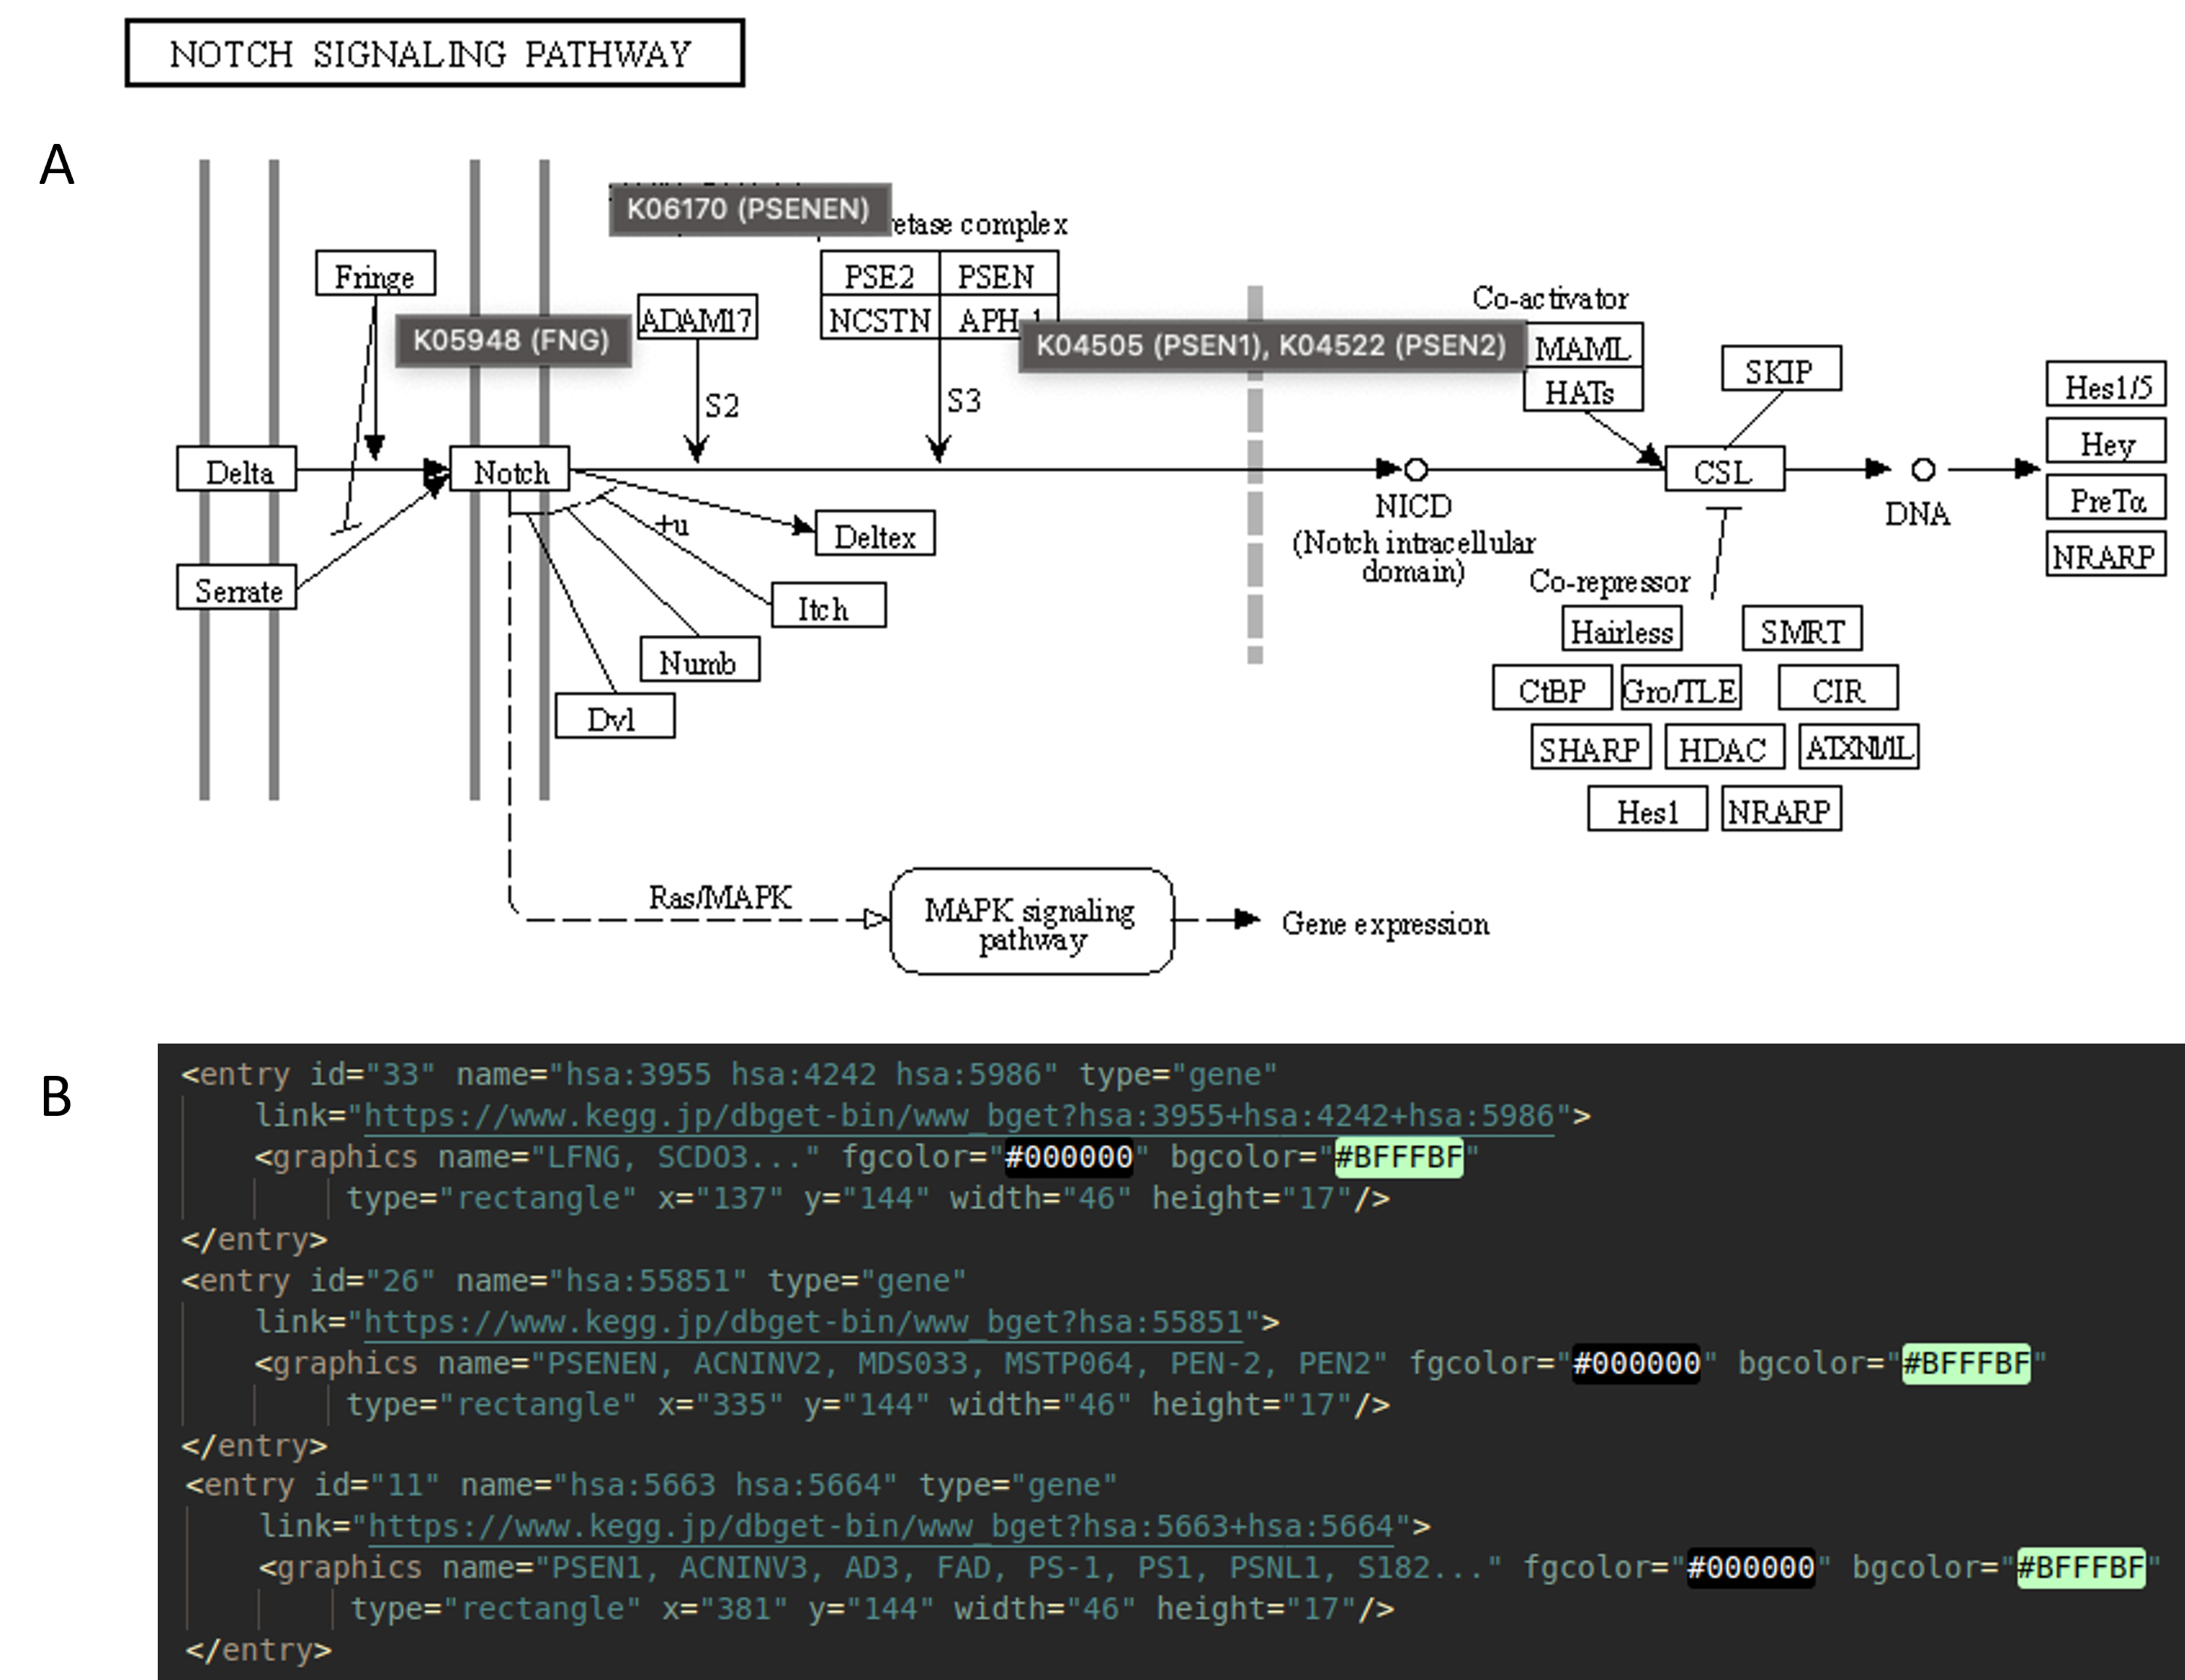
\includegraphics[width=1\textwidth]{figures/corps/figure13.png}
    \caption{Représentation d’une voie KEGG}
    \label{fig:13_kegg}
\end{figure}
Légende : A. La représentation graphique d’une voie de signalisation KEGG sur la page internet avec l’exemple de la voie Notch. Chaque rectangle représente un gène et les flèches une interaction ($\rightarrow$ activation, $\dashv$ inhibition). Les protéines représentées en bloc forment des complexes protéiques. B. Un extrait de cette même voie en format fichier .xml. Chaque gène est représenté par une balise « \textit{entry} » comprenant un identifiant, un nom et un type. 

\begin{table}[H]
\caption{Caractéristiques des voies de signalisation étudiées}
\label{table:voiecaracteristiq}
\rowcolors{2}{lightgray!80!lightgray!50}{lightgray!70!lightgray!40}
\footnotesize{}
\begin{adjustbox}{center}
\begin{tabular}{|l|l|l|l|l|l|l|}\hline
\rowcolor{lightgray}\textbf{Nom de la voie} & \textbf{Catégorie KEGG}  & \textbf{\begin{tabular}[c]{@{}l@{}}Nombre \\ de gènes \\ dans la \\ voie\end{tabular}} & \textbf{\begin{tabular}[c]{@{}l@{}}Nombre \\ d'interactions\\ gene-gene\end{tabular}} & \textbf{\begin{tabular}[c]{@{}l@{}}Nombre\\ de sous-\\ voie\end{tabular}} & \textbf{\begin{tabular}[c]{@{}l@{}}Nombre de\\ gènes dans \\ la plus \\ grande \\ sous-voie\end{tabular}} & \textbf{\begin{tabular}[c]{@{}l@{}}Etendue des\\ moments des \\ naissances des \\ gènes\end{tabular}} \\\hline
p53                     & Cell growth and death           & 64   & 70  & 254   & 7  & {[}1,25{]}  \\\hline
AGE-RAGE                & \begin{tabular}[c]{@{}l@{}}Endocrine and\\ metabolic disease\end{tabular} & 62   & 93  & 358   & 6  & {[}1,24{]}  \\\hline
Adipocytokine           & Endocrine system                & 36   & 48  & 54    & 8  & {[}1,17{]}  \\ 
Estrogen                & Endocrine system                & 62   & 69  & 29    & 16 & {[}2,24{]}  \\  
Glucagon                & Endocrine system                & 50   & 55  & 40    & 9  & {[}1,25{]}  \\   
GnRH                    & Endocrine system                & 41   & 39  & 16    & 16 & {[}1,21{]}  \\  
Insulin                 & Endocrine system                & 62   & 77  & 255   & 11 & {[}1,25{]}  \\  
Ovarian steroidogenesis & Endocrine system                & 45   & 25  & 15    & 6  & {[}1,25{]}  \\   
Oxytocin                & Endocrine system                & 58   & 73  & 51    & 9  & {[}1,21{]}  \\    
PPAR                    & Endocrine system                & 51   & 63  & 61    & 2  & {[}1,23{]}  \\       
Prolactin               & Endocrine system                & 54   & 55  & 63    & 14 & {[}1,25{]}  \\   
Relaxin                 & Endocrine system                & 81   & 103 & 140   & 13 & {[}1,24{]}  \\   
Thyroid hormone         & Endocrine system                & 78   & 85  & 102   & 7  & {[}1,21{]}  \\\hline       
B cell receptor         & Immune system                   & 47   & 57  & 88    & 13 & {[}1,22{]}  \\ 
C-type lectin receptor  & Immune system                   & 154  & 185 & 107   & 8  & {[}1,25{]}  \\            
Chemokine               & Immune system                   & 58   & 82  & 183   & 11 & {[}1,21{]}  \\              
FC epsilon RI           & Immune system                   & 42   & 47  & 42    & 10 & {[}1,24{]}  \\    
IL-17                   & Immune system                   & 91   & 152 & 709   & 9  & {[}1,25{]}  \\  
NOD-like receptor       & Immune system                   & 168  & 164 & 420   & 9  & {[}1,25{]}  \\    
RIG-I-like receptor     & Immune system                   & 53   & 73  & 374   & 8  & {[}1,19{]}  \\    
T cell receptor         & Immune system                   & 66   & 99  & 376   & 9  & {[}1,25{]}  \\                   
Toll-like receptor      & Immune system                   & 79   & 109 & 371   & 10 & {[}1,25{]}  \\\hline  
Neurotrophin            & Nervous system                  & 77   & 117 & 952   & 16 & {[}1,25{]}  \\\hline       
AMPK                    & Signal transduction             & 69   & 67  & 184   & 10 & {[}1,25{]}  \\      
Apelin                  & Signal transduction             & 62   & 78  & 26    & 11 & {[}1,21{]}  \\   
Calcium                 & Signal transduction             & 52   & 67  & 77    & 8  & {[}1,21{]}  \\                  
cAMP                    & Signal transduction             & 88   & 120 & 1966  & 11 & {[}1,24{]}  \\    
cGMP-PKG                & Signal transduction             & 65   & 74  & 201   & 12 & {[}1,25{]}  \\     
ErbB                    & Signal transduction             & 60   & 91  & 309   & 10 & {[}1,19{]}  \\          
FoxO                    & Signal transduction             & 80   & 78  & 70    & 9  & {[}1,25{]}  \\   
Hedgehog                & Signal transduction             & 59   & 50  & 41    & 5  & {[}1,24{]}  \\         
HIF-1                   & Signal transduction             & 65   & 76  & 54    & 7  & {[}1,17{]}  \\     
Hippo                   & Signal transduction             & 91   & 85  & 73    & 6  & {[}1,24{]}  \\     
JAK-STAT                & Signal transduction             & 85   & 262 & 12958 & 12 & {[}1,25{]}  \\        
MAPK                    & Signal transduction             & 119  & 172 & 2083  & 11 & {[}1,21{]}  \\      
mTOR                    & Signal transduction             & 76   & 91  & 375   & 14 & {[}1,16{]}  \\    
NF-Kappa B              & Signal transduction             & 137  & 122 & 110   & 6  & {[}1,24{]}  \\    
Notch                   & Signal transduction             & 25   & 30  & 64    & 4  & {[}1,20{]}  \\          
Phospholipase D         & Signal transduction             & 56   & 71  & 235   & 11 & {[}2,25{]}  \\\hline   
\end{tabular}
\end{adjustbox}
\end{table}\newpage

\textit{Suite du tableau \ref{table:voiecaracteristiq}}
\begin{table}[H]
\rowcolors{2}{lightgray!80!lightgray!50}{lightgray!70!lightgray!40}
\footnotesize{}
\begin{adjustbox}{center}
\begin{tabular}{|l|l|l|l|l|l|l|}\hline
\rowcolor{lightgray}\textbf{Nom de la voie\hspace{1cm}} & \textbf{Catégorie KEGG \hspace{0.3cm}}  & \textbf{\begin{tabular}[c]{@{}l@{}}Nombre \\ de gènes \\ dans la \\ voie\end{tabular}} & \textbf{\begin{tabular}[c]{@{}l@{}}Nombre \\ d'interactions\\ gene-gene\end{tabular}} & \textbf{\begin{tabular}[c]{@{}l@{}}Nombre\\ de sous-\\ voie\end{tabular}} & \textbf{\begin{tabular}[c]{@{}l@{}}Nombre de\\ gènes dans \\ la plus \\ grande \\ sous-voie\end{tabular}} & \textbf{\begin{tabular}[c]{@{}l@{}}Etendue des\\ moments des \\ naissances des \\ gènes\end{tabular}} \\\hline
PI3K-Akt                & Signal transduction             & 90   & 97  & 668   & 13 & {[}1,25{]}  \\     
Rap1                    & Signal transduction             & 80   & 99  & 108   & 5  & {[}1,23{]}  \\   
Ras                     & Signal transduction             & 87   & 112 & 232   & 9  & {[}1,23{]}  \\
Sphingolipid            & Signal transduction             & 63   & 72  & 51    & 6  & {[}1,23{]}  \\  
TGF-Beta                & Signal transduction             & 73   & 76  & 61    & 7  & {[}1,20{]}  \\ 
TNF                     & Signal transduction             & 101  & 54  & 27    & 8  & {[}1,24{]}  \\   
VEGF                    & Signal transduction             & 28   & 34  & 19    & 10 & {[}1,18{]}  \\     
Wnt                     & Signal transduction             & 85   & 98  & 402   & 11 & {[}1,24{]}  \\\hline     
\end{tabular}
\end{adjustbox}
\end{table}
Légende : Ce tableau récapitule les caractéristiques de chacune des 47 voies de signalisation utilisée pour nos deux études. Le nombre de gènes est le nombre de gène unique, les paralogues ne sont pas comptabilisés. L’étendue des moments de naissance des gènes est représentée avec [nœud le plus ancien, nœud le plus récent].

\newpage
\section{Notions supplémentaires : Question de dosage des gènes}
\par Ce chapitre est une partie secondaire à la thèse, mais nécessaire à la compréhension de l’article 3 en Annexe \ref{article3}. 
\par L’une des pressions qui peut régir sur le maintien des gènes en forme dupliquée ou leur retour en singleton peut-être une question de dosage entre deux protéines interagissant ensemble. La question de dosage est directement liée à la quantité d’une protéine dans un organisme, et par extension peut être lié au nombre de copies de gènes nécessaires pour produire une protéine fonctionnelle. Dans la majorité des cas un allèle (un exemplaire d’un gène) suffit pour être fonctionnel. Cependant il existe des cas où la pression de la quantité génique est très importante, notons les gènes haplo-insuffisants, mono-alléliques, soumis à empreinte parentale et du chromosome X. 
\par Les gènes haplo-insuffisants sont des gènes pour lesquels une simple copie du gène n’est pas suffisante pour être fonctionnel. Ce qui sous-entend qu’ils ont besoin d’être au minimum deux pour le devenir. Les gènes haplo-insuffisants, lorsqu’ils ont perdu une de leurs copies peuvent mener à différents phénotypes (individus +/-) \parencite{johnson_causes_2019}. 
\par Au contraire des haplo-insuffisants, les gènes d’expression mono-alléliques ont a priori besoin d’être en une seule copie pour être fonctionnels. Il y a par exemple les protéines immunoglobulines du système immunitaire qui sont présents en plusieurs formes d’allèle dans le génome, seulement un seul allèle à chaîne légère et à chaîne lourde sont activés \parencite{vettermann_allelic_2010}. 
\par Chez les euthériens, les gènes soumis à empreinte parentale sont caractérisés par le fait qu’ils s’expriment uniquement s’ils viennent du père ou de la mère. Quant aux gènes portés par le chromosome X, la majorité sont éteints sur l’un des deux chromosomes, et ce de façon aléatoire, clonale et très tôt chez l’embryon femelle \parencite{balaton_exceptional_2018}. 
Dans notre étude 3, nous nous sommes focalisés sur ces gènes soumis à une pression de dosage pour le clade des téléostéens.


